\chapter{Datenintegrität}

\section{Einführung}

Stellen Sie sich vor, Sie feiern Ihren 18. Geburtstag und wollen Ihren besten Freunden einige Fotos aus Ihrer Kindheit zeigen. Die Fotos sind aber leider alle verpixelt und können nicht richtig angezeigt werden! Oder stellen Sie sich vor, Sie wollen in einigen Jahren Bilder von Ihrem Date anschauen, die Bilder auf Ihrer Festplatte sind jedoch unleserlich. \textit{Bad luck}? Fast genau dies ist dem Profi-Fotografen Tony Northrup geschehen, als er den 18. Geburtstag seiner Tochter mit Fotos aus deren Kindheit feiern wollte: \href{https://www.youtube.com/watch?v=xvbnhCDfREk}{Video}.

Bei der Übertragung von Bits über das Internet können einzelne Bits spontan verändert oder gelöscht werden -- dies kann fatale Folgen haben! Auch gespeicherte Daten können mit der Zeit unbemerkt beschädigt werden: Ändert sich ein gespeichertes Bit spontan von einer 1 zu einer 0 (oder umgekehrt), spricht man von sogenanntem \textit{bit rot}.

Dies sind klassische Beispiele für Fehler, die bei der Speicherung und Übertragung von Daten auftreten können. Mit dem Begriff \enquote{Datenintegrität} bezeichnen wir die Korrektheit und Vollständigkeit von Daten. Datenintegrität ist ein wichtiges Thema in der Informatik, da es darum geht, sicherzustellen, dass Daten während ihrer Speicherung und Übertragung nicht verändert oder beschädigt werden.

\section{Prüfbits}

Buchstaben können auf unterschiedliche Weise kodiert sein -- bei \gls{ASCII} werden beispielsweise sieben Bits pro Zeichen verwendet:

\begin{table}[H]
    \centering
    \begin{tabular}{cc}
        Buchstabe & Kodierung        \\\midrule
        A         & \texttt{1000001} \\\midrule
        B         & \texttt{1000010} \\\midrule
        C         & \texttt{1000011} \\\midrule
        $\cdots$  & $\cdots$
    \end{tabular}
\end{table}
Bei der Datenübertragung können aber einzelne Bits spontan von einem \texttt{1} zu einem \texttt{0} werden (oder umgekehrt). Was könnte getan werden, um dieser Gefahr vorzubeugen?

Ein erster, einfacher Ansatz bestünde darin, jedem Code noch ein weiteres Bit anzuhängen, so dass die Summe der Bits immer gerade ist:

\begin{table}[H]
    \centering
    \begin{tabular}{cc}
        Buchstabe & Kodierung                              \\\midrule
        A         & \texttt{1000001\underline{\textbf{0}}} \\\midrule
        B         & \texttt{1000010\underline{\textbf{0}}} \\\midrule
        C         & \texttt{1000011\underline{\textbf{1}}} \\\midrule
        $\cdots$  & $\cdots$
    \end{tabular}
\end{table}

Wenn sich \textit{ein} Bit nun spontan verändert, wird der Code als fehlerhaft erkannt, da die Summe der Bits, welche den Wert \texttt{1} haben, nicht mehr gerade ist. Ein Computer könnte nun also anfordern, dass der Code nochmals geschickt wird.

Die Idee von Prüfziffern ist, dass jede Prüfziffer nach dem gleichen Prinzip berechnet ist. Stimmt bei einem erhaltenen Code die Formel mit der Prüfziffer nicht überein, wird der Code als fehlerhaft erkannt.
\begin{myexercise}
    Folgende Prüfziffern sind alle nach der gleichen Regel berechnet. Können Sie die Regel erkennen?
    \begin{itemize}
        \item 31\textbf{6}
        \item 1298\textbf{0}
        \item 3333574\textbf{2}
        \item 2\textbf{8}
        \item 10\textbf{9}
    \end{itemize}
    Was wäre die Kontrollziffer für die Zahl 4163?

    \begin{myanswer}
        \[3 + 1 + 6 = 10\]
        \[1 + 2 + 9 + 8 + 0 = 20\]
        \[3 + 3 + 3 + 3 + 5 + 7 + 4 + 2=30\]
        etc.
        Für die Zahl 4163: 4163\textbf{6}
    \end{myanswer}
\end{myexercise}

Die \gls{EAN} ist ein Standard für die Kodierung von Waren. Fast alle käuflich erhältlichen Waren auf dem Markt enthalten einen solchen Code, welcher aus 13 Ziffern besteht. Häufig wird er in Form eines Strichcodes dargestellt, wobei zwei Striche eine Ziffer darstellen. Dazu kommen drei Begrenzungszeichen aus je zwei Strichen: das Start-, das Trenn- und das Stoppzeichen (siehe \cref{fig:ean}).

\begin{figure}[H]
    \centering
    \includegraphics[width=0.7\linewidth]{Grundlagen_Info/05_Datenintegritaet/Figures/EAN}
    \caption{Bestandteile eines \gls{EAN}}
    \label{fig:ean}
\end{figure}

Ein \gls{EAN} besteht aus 12 Ziffern und einer Prüfziffer:
\begin{equation}\label{eq:ean}
    x_1x_2x_3x_4x_5x_6x_7x_8x_9x_{10}x_{11}x_{12}\textcolor{red}{x_{13}}
\end{equation}


Das Scannen eines falschen Codes könnte zu falschen Preisen an der Kasse führen, weshalb \gls{EAN} ebenfalls eine Prüfziffer enthalten, die sich wie folgt berechnet:

\begin{enumerate}
    \item $s=x_1+x_3+ x_5+ x_7+ x_9+ x_{11}+3\times( x_2+ x_4+ x_6+ x_8+ x_{10}+ x_{12})$
    \item Anschliessend wird $\textcolor{red}{x_{13}}$ so gewählt, dass $s+\textcolor{red}{x_{13}}$ durch 10 teilbar ist.
\end{enumerate}


\begin{myexercise}
    Welche folgender Fehler werden durch einen \gls{EAN} erkannt?
    \begin{itemize}
        \item Vertippen (eine Ziffer ist falsch)
        \item Vertauschen zweier benachbarter Ziffern
        \item Auslassen (eine Ziffer wird vergessen)
        \item 2 mal Vertippen $\rightarrow$ 2 Ziffern werden falsch getippt
    \end{itemize}
    \begin{myanswer}
        \begin{itemize}
            \item \textbf{Vertippen:} wird immer erkannt. Ändert sich eine Ziffer um $d$ ($1 \leq |d| \leq 9$), ändert sich $s$ um $d$ (Gewicht 1) bzw. um $3d$ (Gewicht 3). Beides ist nie ein Vielfaches von 10, die Prüfziffer passt also nicht mehr.
            \item \textbf{Vertauschen zweier benachbarter Ziffern:} wird meistens, aber nicht immer erkannt. Unterscheiden sich die beiden Ziffern um 5 (z.B. 0 und 5), ändert sich $s$ um $\pm 10$, und der Fehler bleibt unbemerkt (siehe \cref{ex:ean}).
            \item \textbf{Auslassen:} wird erkannt, da der Code dann nur noch 12 statt 13 Ziffern hat und somit kein gültiger \gls{EAN} mehr ist.
            \item \textbf{2 mal Vertippen:} wird nicht immer erkannt, da sich zwei Fehler gegenseitig aufheben können. Wird z.B. an Position 1 (Gewicht 1) eine Ziffer um 3 zu gross und an Position 3 (Gewicht 1) eine Ziffer um 3 zu klein getippt, bleibt $s$ gleich.
        \end{itemize}
    \end{myanswer}
\end{myexercise}

\begin{myexercise}
    Berechnen Sie für 978314221213 die \acrshort{EAN}-13-Prüfziffer.
    \begin{myanswer}
        5
    \end{myanswer}
\end{myexercise}

\begin{myexercise}\label{ex:ean}
    Bestimmen Sie für den folgenden \gls{EAN}-Code alle Paare von benachbarten Ziffern, deren Austausch in der Reihenfolge nicht erkannt werden kann:
    \begin{alltt}
        4\(\underset{\makebox[\widthof{\texttt{X}}][c]{\footnotesize\texttt{\red{2}}}}{\texttt{\red{0}}}\)3\(\underset{\makebox[\widthof{\texttt{X}}][c]{\footnotesize\texttt{\red{4}}}}{\texttt{\red{0}}}\)5\(\underset{\makebox[\widthof{\texttt{X}}][c]{\footnotesize\texttt{\red{6}}}}{\texttt{\red{3}}}\)8\(\underset{\makebox[\widthof{\texttt{X}}][c]{\footnotesize\texttt{\red{8}}}}{\texttt{\red{6}}}\)5\(\underset{\makebox[\widthof{\texttt{X}}][c]{\footnotesize\texttt{\red{10}}}}{\texttt{\red{7}}}\)4\(\underset{\makebox[\widthof{\texttt{X}}][c]{\footnotesize\texttt{\red{12}}}}{\texttt{\red{6}}}\)5
    \end{alltt}
    Die kleinen roten Zahlen unter dem Code gehören nicht zum Code. Sie markieren die geraden Positionen 2, 4, \ldots, 12, deren Ziffern gemäss \cref{eq:ean} mit 3 gewichtet werden.
    \begin{myanswer}
        Damit ein Austausch zweier benachbarter Ziffern nicht entdeckt würde, müsste sich die Summe $s$ um ein Vielfaches von 10 (oder 0) ändern. Dies wäre beispielsweise der Fall, wenn die zwei Ziffern 3 und 8 (Positionen 6 und 7) vertauscht würden.

        Der Beitrag der Ziffern zu $s$ im ursprünglichen und im abgeänderten Code sind in folgender Tabelle aufgelistet:


        \begin{table}[H]
            \centering
            \begin{tabular}{lp{3cm}p{4cm}l}
                \textbf{Position} & \textbf{Ziffer} & \textbf{Gewichtung\newline (siehe \cref{eq:ean})} & \textbf{Beitrag zu $s$} \\
                \midrule
                6                 & 3               & 3                                              & 9                       \\
                7                 & 8               & 1                                              & 8                       \\
            \end{tabular}
        \end{table}
        \[\Downarrow\]
        \begin{table}[H]
            \centering
            \begin{tabular}{lp{3cm}p{4cm}l}
                \textbf{Position} & \textbf{Ziffer\newline (vertauscht)} & \textbf{Gewichtung\newline (siehe \cref{eq:ean})} & \textbf{Beitrag zu $s$} \\
                \midrule
                6                 & 8                                    & 3                                              & 24                      \\
                7                 & 3                                    & 1                                              & 3                       \\
            \end{tabular}
        \end{table}

        Die Summe $s$ ändert sich also um:
        \[
            (24 + 3) - (9 + 8) = 27 - 17 = +10
        \]

        Da sich $s$ um ein Vielfaches von 10 verändert, bleibt die Prüfziffer gleich, und der Fehler wird nicht entdeckt.

        Dasselbe würde auch mit Positionen 4 und 5 (Ziffern 0 und 5) funktionieren.
    \end{myanswer}

\end{myexercise}

\begin{mychallenge}
    Begründen Sie allgemein, für welche Arten von Ziffern ein Vertauschen zweier benachbarter Ziffern in einer \gls{EAN}-Prüfziffer nicht entdeckt wird.
    \begin{myanswer}
        Damit ein Austausch zweier benachbarter Ziffern nicht entdeckt wird, darf sich die gewichtete Summe $s$ nicht ändern, da die Prüfziffer $x_{13}$ so gewählt ist, dass
        \[
            s + x_{13} \equiv 0 \mod 10
        \]
        gilt.

        Wir bezeichnen die beiden benachbarten Ziffern mit $a$ und $b$ an den Positionen $i$ und $i+1$. Die zugehörigen Gewichte im \gls{EAN}-System sind alternierend 1 und 3, also entweder $(g_i, g_{i+1}) = (1, 3)$ oder $(3, 1)$.

        Der ursprüngliche Beitrag dieser beiden Ziffern zur Summe $s$ ist:
        \[
            s_\text{alt} = g_i \cdot a + g_{i+1} \cdot b
        \]

        Nach dem Vertauschen lautet der Beitrag:
        \[
            s_\text{neu} = g_i \cdot b + g_{i+1} \cdot a
        \]

        Die Änderung der Summe beträgt also:
        \[
            \Delta s = s_\text{neu} - s_\text{alt} = g_i \cdot b + g_{i+1} \cdot a - (g_i \cdot a + g_{i+1} \cdot b)
            = (g_i - g_{i+1})(b - a)
        \]

        Da $g_i$ und $g_{i+1}$ abwechselnd $1$ und $3$ sind, ist $g_i - g_{i+1} \in \{-2, +2\}$. Es ergibt sich also:
        \[
            \Delta s = \pm 2 (b - a)
        \]

        Diese Änderung bleibt genau dann unbemerkt, wenn $\Delta s \equiv 0 \mod 10$ ist, also:
        \[
            \pm 2(b - a) \equiv 0 \mod 10 \quad \Leftrightarrow \quad b - a \equiv 0 \mod 5
        \]

        Es folgt:
        \[
            |b - a| \in \{0, 5\}
        \]

        Der Fall $b = a$ ist trivial, da keine Vertauschung erfolgt. Für eine echte Vertauschung mit $|b - a| = 5$ wird der Fehler \emph{nicht erkannt}.

        \medskip

        \textbf{Fazit:} Ein Vertauschen zweier benachbarter Ziffern im \gls{EAN}-Code bleibt genau dann unentdeckt, wenn sich ihre Werte um 5 unterscheiden, also $|b - a| = 5$ gilt.

    \end{myanswer}
\end{mychallenge}

\begin{mychallenge}
    In dieser Challenge untersuchen Sie zwei Alternativen zum \gls{EAN}-Code. Die Prüfziffer $x_{13}$ wird jeweils wieder so gewählt, dass $s+x_{13}$ durch 10 teilbar ist, nur die Berechnung von $s$ ändert sich:
    \begin{aenum}
        \item $s=x_1+x_3+ x_5+ x_7+ x_9+ x_{11}+\textcolor{red}{5}\times( x_2+ x_4+ x_6+ x_8+ x_{10}+ x_{12})$

              Begründen Sie, wieso diese Alternative ein Vertippen nicht zuverlässig erkennt.
        \item $s=x_1+x_3+ x_5+ x_7+ x_9+ x_{11}+\textcolor{red}{4}\times( x_2+ x_4+ x_6+ x_8+ x_{10}+ x_{12})$

              Erklären Sie, wieso diese Alternative ein Vertippen nicht zuverlässig erkennt, ein Vertauschen benachbarter Ziffern hingegen schon.
    \end{aenum}
    \begin{myanswer}
        \begin{aenum}
            \item Wenn der Vertipper an einer geraden Position geschieht und sich die Ziffer um eine gerade Zahl ändert, ändert sich $s$ um ein Vielfaches von 10. Das wird in dieser Variante nicht erkannt.
            \item Wenn der Vertipper an einer geraden Position geschieht und sich die Ziffer um 5 ändert, ändert sich $s$ um $\pm 20$. Das wird in dieser Variante nicht erkannt.

                  Wenn benachbarte Ziffern vertauscht werden, ändert sich die Summe $s$ um das Dreifache der Differenz $d$ der beiden Ziffern. Wenn $d=0$ ist, sind die Ziffern gleich und ein Vertauschen hat keinen Einfluss. Für alle anderen $|d|\in\{1, \dots, 9\}$ ist $3d$ nicht durch 10 teilbar, wodurch sich die Prüfziffer ändern müsste. Vertauschen wird also in jedem Fall erkannt.
        \end{aenum}
    \end{myanswer}
\end{mychallenge}

\begin{myexercise}
    Nehmen wir an, dass an der vierten Position im Code aus \cref{ex:ean} eine 8 statt der 0 getippt wurde. Finden Sie mindestens 5 Möglichkeiten, an anderen Stellen den Fehler so zu machen, dass die fehlerhafte Darstellung einem \gls{EAN}-Code entspricht und somit dieser Doppelfehler unbemerkt bleibt.
    \begin{myanswer}
        Die Ziffer an Position 4 wurde von 0 auf 8 geändert. Da Position 4 das Gewicht 3 hat, verändert sich die Summe $s$ um
        \[
            (8-0) \cdot 3 = +24
        \]
        Damit der Doppelfehler unbemerkt bleibt, muss an einer anderen Stelle ein Fehler mit dem Beitrag $-24$, $-14$, $-4$, $+6$, $+16$ etc. gemacht werden. In diesem Fall verändert sich $s$ um 0, +10, +20, +30 etc., sodass $x_{13}$ gleich bleibt.

        Dies könnte mit folgenden möglichen Änderungen erfolgen:
        \begin{center}
            \begin{tabular}{lllll}
                \textbf{Position} & \textbf{Gewicht} & \textbf{Änderung} & \textbf{Fehlerbeitrag} & \textbf{Gesamt-Fehler} \\
                \midrule
                1                 & 1                & 4 $\rightarrow$ 0 & $-4$                   & $24-4=20$              \\\midrule
                2                 & 3                & 0 $\rightarrow$ 2 & $+6$                   & $24+6=30$              \\\midrule
                3                 & 1                & 3 $\rightarrow$ 9 & $+6$                   & $24+6=30$              \\\midrule
                9                 & 1                & 5 $\rightarrow$ 1 & $-4$                   & $24-4=20$              \\\midrule
                10                & 3                & 7 $\rightarrow$ 9 & $+6$                   & $24+6=30$              \\
            \end{tabular}
        \end{center}

        In all diesen Fällen bleibt die Prüfziffer $x_{13}$ unverändert, der Doppelfehler wird also nicht erkannt.

    \end{myanswer}
\end{myexercise}

\begin{myexercise}
    Die ursprünglichen \gls{ISBN}-10-Codes zur eindeutigen Bezeichnung von Büchern bestanden aus 9 Ziffern und einem Prüfsymbol aus den folgenden Symbolen:

    \texttt{\{0, 1, 2, 3, 4, 5, 6, 7, 8, 9, X\}}

    wobei \texttt{X} die Zahl 10 repräsentierte. Für die neun Ziffern $x_1$, $x_2$, $\cdots$, $x_9$, hat man das Prüfsymbol $x_{10}$ wie folgt bestimmt:
    \[10\times x_1+9\times x_2+8\times x_3+\cdots+2\times x_9 + x_{10}\]
    ist ein Vielfaches von 11. Falls $x_{10} = 10$ ist das Prüfsymbol \texttt{X}.
    \begin{enumerate}
        \item Bestimmen Sie für die folgenden Symbolfolgen, welche \gls{ISBN}-10-Codes sind und welche es nicht sind:
              \begin{itemize}
                  \item \texttt{020144124\textbf{1}}
                  \item \texttt{270004302\textbf{X}}
                  \item \texttt{809004048\textbf{9}}
                  \item \texttt{010144124\textbf{X}}
              \end{itemize}
        \item Die neunstellige Zahl eines Buches ist \texttt{354042278}. Bestimmen Sie das Prüfsymbol des \gls{ISBN}-10-Codes des Buches.
    \end{enumerate}
    \begin{myanswer}
        \textbf{a) Prüfung der Symbolfolgen}

        Zur Erinnerung: Ein \gls{ISBN}-10-Code ist gültig, wenn die gewichtete Summe
        \[
            10x_1 + 9x_2 + 8x_3 + \cdots + 2x_9 + x_{10} \equiv 0 \mod 11
        \]
        ist.

        Aufgabe (a): Wenn wir diese Formel anwenden, finden wir heraus, dass alle ausser dem zweiten Code gültige \gls{ISBN}-Codes sind.

        Aufgabe (b): $3*10+5*9+4*8+0*7+4*6+2*5+2*4+7*3+8*2=186 \rightarrow x_{10}=1$, da $187=11*17$.

    \end{myanswer}

\end{myexercise}

\section{Fehler erkennen und korrigieren}

Sie kennen Fehlererkennung bereits aus Ihrem Alltag: So beispielsweise bei der Rechtschreibprüfung in Word, die Ihnen das korrekte Wort vorschlägt (siehe \cref{fig:word}).

\begin{figure}[H]
    \centering
    \includegraphics[width=0.7\linewidth]{Grundlagen_Info/05_Datenintegritaet/Figures/Word}
    \caption{Rechtschreibprüfung im Programm Microsoft Word}
    \label{fig:word}
\end{figure}

\begin{myexample}\label{ex:word}
Wie viele Tippfehler werden im Beispiel aus \cref{fig:word} in jedem Fall erkannt?

Im gezeigten Beispiel wird ein Tippfehler noch erkannt. Garantiert erkannt wird jedoch nicht einmal ein einzelner Tippfehler: Wird aus dem ursprünglich gemeinten Wort \enquote{Fehler} durch einen Tippfehler das Wort \enquote{Fehlen}, entsteht wieder ein korrektes Wort, und der Fehler bleibt unbemerkt. Zudem kann nicht jeder erkannte Tippfehler eindeutig korrigiert werden: Ein Tippfehler vom Wort \enquote{Fehler} hin zu \enquote{Zehler} wird zwar erkannt, doch \enquote{Zehler} hat sowohl einen Buchstaben Abstand zum (korrekten, beabsichtigten) Wort \enquote{Fehler} wie auch zum (nicht beabsichtigten, aber korrekten) Wort \enquote{Zähler}.
\end{myexample}

Was können wir aus \cref{ex:word} lernen? Damit ein Fehler automatisch korrigiert werden kann, muss der Unterschied zwischen dem vertippten Wort und allen anderen möglichen Wörtern grösser sein als der Abstand zum ursprünglichen Wort.

Im Folgenden unterscheiden wir zwischen \textbf{k-fehler\-erkennenden} sowie \textbf{k-fehler\-korrigierenden} Kodierungen. Eine Kodierung heisst \textbf{k-fehlererkennend}, wenn das Umflippen von 1, 2, $\cdots$ bis und mit \textbf{k} Bits in der Nachricht als Fehler erkannt wird. Falls bis zu \textbf{k} Fehler nicht nur erkannt, sondern auch behoben werden können, spricht man von \textbf{k-fehlerkorrigierenden Kodierungen}.

\begin{myexample}\label{ex:code-kerk}
\cref{tab:codes} zeigt, wie eine Nachricht so kodiert werden kann, dass Fehler erkannt werden:
\begin{itemize}
    \item In Kodierung 1 handelt es sich schlicht und einfach um die ursprüngliche Nachricht.
    \item In Kodierung 2 wird die ursprüngliche Nachricht verdreifacht.
    \item In Kodierung 3 wird die ursprüngliche Nachricht verdoppelt, dazu kommt ein \textbf{Paritätsbit} (\underline{unterstrichen}) am Ende der Nachricht.
\end{itemize}
\begin{table}[H]
    \centering
    \begin{tabular}{cccc}
                         & \textbf{Kodierung$_1$} & \textbf{Kodierung$_2$}     & \textbf{Kodierung$_3$}                \\
        \midrule
        \textbf{Weiss}   & 00                     & 00\textcolor{orange}{0000} & 00\textcolor{orange}{00\underline{0}} \\
        \midrule
        \textbf{Gelb}    & 01                     & 01\textcolor{orange}{0101} & 01\textcolor{orange}{01\underline{1}} \\
        \midrule
        \textbf{Blau}    & 10                     & 10\textcolor{orange}{1010} & 10\textcolor{orange}{10\underline{1}} \\
        \midrule
        \textbf{Schwarz} & 11                     & 11\textcolor{orange}{1111} & 11\textcolor{orange}{11\underline{0}} \\
    \end{tabular}
    \caption{Kodierungstabelle}
    \label{tab:codes}
\end{table}

Wie viele Fehler werden durch die unterschiedlichen Kodierungen bestimmt erkannt?
\begin{itemize}
    \item In der ursprünglichen Kodierung können Fehler nicht erkannt werden. Wird beispielsweise Weiss (\texttt{00}) fälschlicherweise als \texttt{01} versandt, geht der Empfänger davon aus, dass Gelb gesandt wurde und erkennt keine Fehler.
    \item In der zweiten Kodierung werden bis zu zwei Fehler erkannt, da es mindestens drei \enquote{Mutationen} benötigt, um zu einem anderen Code zu werden.
    \item Bei der dritten Kodierung verhält es sich ebenso wie bei der zweiten.
\end{itemize}
Kodierung$_2$ und Kodierung$_3$ sind also betreffend Fehlererkennung gleich gut, allerdings ist Kodierung$_3$ kürzer und daher zu bevorzugen.
\end{myexample}

Um zu bestimmen, wie viele Fehler eine bestimmte Kodierung erkennen kann, müssen wir uns die Abstände zwischen allen möglichen Code-Wörtern anschauen.

\begin{myexample}\label{ex:abstand}
Angenommen, wir hätten drei Code-Wörter, \texttt{ANNA}, \texttt{ENZO} und \texttt{HANS}, dann könnten die Abstände zwischen allen Code-Wörtern wie folgt bestimmt werden:

\begin{table}[H]
    \centering
    \begin{tabular}{c@{\hspace{1.5cm}}c@{\hspace{1.5cm}}c}
        \begin{tabular}{c}
            \texttt{A N N A} \\
            \texttt{E N Z O} \\ \hline
            \texttt{x o x x} \\
            \textcolor{orange}{Abstand 3}
        \end{tabular}
         &
        \begin{tabular}{c}
            \texttt{A N N A} \\
            \texttt{H A N S} \\ \hline
            \texttt{x x o x} \\
            \textcolor{orange}{Abstand 3}
        \end{tabular}
         &
        \begin{tabular}{c}
            \texttt{E N Z O} \\
            \texttt{H A N S} \\ \hline
            \texttt{x x x x} \\
            \textcolor{orange}{Abstand 4}
        \end{tabular}
    \end{tabular}
    \caption{Abstände zwischen den Codewörtern \texttt{ANNA}, \texttt{ENZO} und \texttt{HANS}}
    \label{tab:hans}
\end{table}

Die \enquote{\texttt{x}} bezeichnen Stellen, an denen sich die Buchstaben unterscheiden und die \enquote{\texttt{o}} Stellen, an denen die Buchstaben gleich sind. Der Abstand zwischen einem Wort-Paar ergibt sich aus der Summe der \enquote{\texttt{x}}.

Der minimale Abstand in diesem Beispiel ist 3, daher könnten in dieser Kodierung bis zu 2 Fehler, bzw. \enquote{Mutationen} erkannt werden. \texttt{ANNA} $\rightarrow$ \texttt{AN\textcolor{red}{Z}A} würde als Fehler erkannt, \texttt{ANNA} $\rightarrow$ \texttt{\textcolor{red}{E}N\textcolor{red}{ZO}} jedoch nicht, da \texttt{ENZO} ein korrektes Code-Wort ist.
\end{myexample}

Binär funktioniert die Abstandsbestimmung genau gleich wie in \cref{ex:abstand}.

\begin{myexample}\label{ex:bin}
Basierend auf Kodierung$_2$ aus \cref{tab:codes} könnten die Abstände zwischen allen Code-Wörtern wie folgt bestimmt werden:

\begin{table}[H]
    \centering
    \begin{tabular}{c@{\hspace{1.5cm}}c@{\hspace{1.5cm}}c}
        \begin{tabular}{c}
            \texttt{0 0 0 0 0 0} \\
            \texttt{0 1 0 1 0 1} \\ \hline
            \texttt{o x o x o x} \\
            \textcolor{orange}{Abstand 3}
        \end{tabular}
         &
        \begin{tabular}{c}
            \texttt{0 0 0 0 0 0} \\
            \texttt{1 0 1 0 1 0} \\ \hline
            \texttt{x o x o x o} \\
            \textcolor{orange}{Abstand 3}
        \end{tabular}
         &
        \begin{tabular}{c}
            \texttt{0 0 0 0 0 0} \\
            \texttt{1 1 1 1 1 1} \\ \hline
            \texttt{x x x x x x} \\
            \textcolor{orange}{Abstand 6}
        \end{tabular} \\
        \begin{tabular}{c}
            \texttt{0 1 0 1 0 1} \\
            \texttt{1 0 1 0 1 0} \\ \hline
            \texttt{x x x x x x} \\
            \textcolor{orange}{Abstand 6}
        \end{tabular}
         &
        \begin{tabular}{c}
            \texttt{0 1 0 1 0 1} \\
            \texttt{1 1 1 1 1 1} \\ \hline
            \texttt{x o x o x o} \\
            \textcolor{orange}{Abstand 3}
        \end{tabular}
         &                            \\
        \begin{tabular}{c}
            \texttt{1 0 1 0 1 0} \\
            \texttt{1 1 1 1 1 1} \\ \hline
            \texttt{o x o x o x} \\
            \textcolor{orange}{Abstand 3}
        \end{tabular}
         &
         &                            \\
    \end{tabular}
    \caption{Abstände zwischen allen Codewörtern der Kodierung$_2$ aus \cref{tab:codes}}
    \label{tab:abst-codes}
\end{table}

Damit können auch in diesem Beispiel bis zu 2 Fehler erkannt werden.
\end{myexample}

\begin{myexercise}\label{ex:xavier}
    Xavier schlägt vor, die Code-Wörter für die Farben aus \cref{ex:code-kerk} anders zu konstruieren. Man soll zu den Darstellungen (zwei Bits, z.B. 11) der Farben das Prüfbit anhängen (z.B. 11\underline{0}), sodass die Anzahl der Einsen gerade wird. Danach sollte man diese drei Bits in zwei Kopien (z.B. 11\underline{0}11\underline{0} für \enquote{Schwarz}) zu einem Code-Wort machen. Konstruieren Sie alle Code-Wörter der Kodierung und bestimmen Sie, wie viele Fehler man damit erkennen kann.
    \begin{myanswer}
        \begin{table}[H]
            \centering
            \begin{tabular}{c@{\hspace{1.5cm}}c@{\hspace{1.5cm}}c}
                \begin{tabular}{c}
                    \texttt{0 0 0 0 0 0} \\
                    \texttt{0 1 1 0 1 1} \\ \hline
                    \texttt{o x x o x x} \\
                    \textcolor{orange}{Abstand 4}
                \end{tabular}
                 &
                \begin{tabular}{c}
                    \texttt{0 0 0 0 0 0} \\
                    \texttt{1 0 1 1 0 1} \\ \hline
                    \texttt{x o x x o x} \\
                    \textcolor{orange}{Abstand 4}
                \end{tabular}
                 &
                \begin{tabular}{c}
                    \texttt{0 0 0 0 0 0} \\
                    \texttt{1 1 0 1 1 0} \\ \hline
                    \texttt{x x o x x o} \\
                    \textcolor{orange}{Abstand 4}
                \end{tabular} \\
                \begin{tabular}{c}
                    \texttt{0 1 1 0 1 1} \\
                    \texttt{1 0 1 1 0 1} \\ \hline
                    \texttt{x x o x x o} \\
                    \textcolor{orange}{Abstand 4}
                \end{tabular}
                 &
                \begin{tabular}{c}
                    \texttt{0 1 1 0 1 1} \\
                    \texttt{1 1 0 1 1 0} \\ \hline
                    \texttt{x o x x o x} \\
                    \textcolor{orange}{Abstand 4}
                \end{tabular}
                 &                            \\
                \begin{tabular}{c}
                    \texttt{1 0 1 1 0 1} \\
                    \texttt{1 1 0 1 1 0} \\ \hline
                    \texttt{o x x o x x} \\
                    \textcolor{orange}{Abstand 4}
                \end{tabular}
                 &
                 &                            \\
            \end{tabular}
            \caption{Abstände zwischen allen Codewörtern der Kodierung von Xavier}
            \label{tab:abst-codes-xavier}
        \end{table}
        Da der Mindestabstand zwischen allen Kodewörtern 4 ist, können bis zu 3 Fehler erkannt werden.
    \end{myanswer}
\end{myexercise}

\begin{myexercise}\label{ex:fehler-kodierungen}
    Bestimmen Sie, wie viele Fehler jede der folgenden Kodierungen erkennen kann. Bestimmen Sie dazu als Erstes den Mindest-Abstand innerhalb jeder Kodierung:
    \begin{table}[H]
        \centering
        \begin{tabular}{ccccc}
                             & \textbf{4-Kopien} & \textbf{Xavier} & \textbf{1-Parity} & \textbf{0-Parity} \\
            \midrule
            \textbf{Weiss}   & \texttt{00000000} & \texttt{000000} & \texttt{000}      & \texttt{001}      \\
            \midrule
            \textbf{Gelb}    & \texttt{01010101} & \texttt{011011} & \texttt{011}      & \texttt{010}      \\
            \midrule
            \textbf{Blau}    & \texttt{10101010} & \texttt{101101} & \texttt{101}      & \texttt{100}      \\
            \midrule
            \textbf{Schwarz} & \texttt{11111111} & \texttt{110110} & \texttt{110}      & \texttt{111}      \\
        \end{tabular}
        \caption{Kodierungstabelle}
        \label{tab:kodierung}
    \end{table}
    \begin{myanswer}
        \begin{table}[H]
            \centering
            \begin{tabular}{c@{\hspace{1.5cm}}c@{\hspace{1.5cm}}c}
                \begin{tabular}{c}
                    \texttt{0 0 0 0 0 0 0 0} \\
                    \texttt{0 1 0 1 0 1 0 1} \\ \hline
                    \texttt{o x o x o x o x} \\
                    \textcolor{orange}{Abstand 4}
                \end{tabular}
                 &
                \begin{tabular}{c}
                    \texttt{0 0 0 0 0 0 0 0} \\
                    \texttt{1 0 1 0 1 0 1 0} \\ \hline
                    \texttt{x o x o x o x o} \\
                    \textcolor{orange}{Abstand 4}
                \end{tabular}
                 &
                \begin{tabular}{c}
                    \texttt{0 0 0 0 0 0 0 0} \\
                    \texttt{1 1 1 1 1 1 1 1} \\ \hline
                    \texttt{x x x x x x x x} \\
                    \textcolor{orange}{Abstand 8}
                \end{tabular} \\
                \begin{tabular}{c}
                    \texttt{0 1 0 1 0 1 0 1} \\
                    \texttt{1 0 1 0 1 0 1 0} \\ \hline
                    \texttt{x x x x x x x x} \\
                    \textcolor{orange}{Abstand 8}
                \end{tabular}
                 &
                \begin{tabular}{c}
                    \texttt{0 1 0 1 0 1 0 1} \\
                    \texttt{1 1 1 1 1 1 1 1} \\ \hline
                    \texttt{x o x o x o x o} \\
                    \textcolor{orange}{Abstand 4}
                \end{tabular}
                 &                                \\
                \begin{tabular}{c}
                    \texttt{1 0 1 0 1 0 1 0} \\
                    \texttt{1 1 1 1 1 1 1 1} \\ \hline
                    \texttt{o x o x o x o x} \\
                    \textcolor{orange}{Abstand 4}
                \end{tabular}
                 &
                 &                                \\
            \end{tabular}
            \caption{Abstände zwischen allen Codewörtern der 4-Kopien-Kodierung}
            \label{tab:abst-4kopien}
        \end{table}
    \end{myanswer}
    \begin{myanswer}
        Kodierung von Xavier: s. Lösungen zu \cref{ex:xavier}.
    \end{myanswer}
    \begin{myanswer}
        \begin{table}[H]
            \centering
            \begin{tabular}{c@{\hspace{1.5cm}}c@{\hspace{1.5cm}}c}
                \begin{tabular}{c}
                    \texttt{0 0 0} \\
                    \texttt{0 1 1} \\ \hline
                    \texttt{o x x} \\
                    \textcolor{orange}{Abstand 2}
                \end{tabular}
                 &
                \begin{tabular}{c}
                    \texttt{0 0 0} \\
                    \texttt{1 0 1} \\ \hline
                    \texttt{x o x} \\
                    \textcolor{orange}{Abstand 2}
                \end{tabular}
                 &
                \begin{tabular}{c}
                    \texttt{0 0 0} \\
                    \texttt{1 1 0} \\ \hline
                    \texttt{x x o} \\
                    \textcolor{orange}{Abstand 2}
                \end{tabular} \\
                \begin{tabular}{c}
                    \texttt{0 1 1} \\
                    \texttt{1 0 1} \\ \hline
                    \texttt{x x o} \\
                    \textcolor{orange}{Abstand 2}
                \end{tabular}
                 &
                \begin{tabular}{c}
                    \texttt{0 1 1} \\
                    \texttt{1 1 0} \\ \hline
                    \texttt{x o x} \\
                    \textcolor{orange}{Abstand 2}
                \end{tabular}
                 &                           \\
                \begin{tabular}{c}
                    \texttt{1 0 1} \\
                    \texttt{1 1 0} \\ \hline
                    \texttt{o x x} \\
                    \textcolor{orange}{Abstand 2}
                \end{tabular}
                 &
                 &                           \\
            \end{tabular}
            \caption{Abstände zwischen allen Codewörtern der 1-Parity-Kodierung}
            \label{tab:abst-1parity}
        \end{table}
    \end{myanswer}
    \begin{myanswer}
        \begin{table}[H]
            \centering
            \begin{tabular}{c@{\hspace{1.5cm}}c@{\hspace{1.5cm}}c}
                \begin{tabular}{c}
                    \texttt{0 0 1} \\
                    \texttt{0 1 0} \\ \hline
                    \texttt{o x x} \\
                    \textcolor{orange}{Abstand 2}
                \end{tabular}
                 &
                \begin{tabular}{c}
                    \texttt{0 0 1} \\
                    \texttt{1 0 0} \\ \hline
                    \texttt{x o x} \\
                    \textcolor{orange}{Abstand 2}
                \end{tabular}
                 &
                \begin{tabular}{c}
                    \texttt{0 0 1} \\
                    \texttt{1 1 1} \\ \hline
                    \texttt{x x o} \\
                    \textcolor{orange}{Abstand 2}
                \end{tabular} \\
                \begin{tabular}{c}
                    \texttt{0 1 0} \\
                    \texttt{1 0 0} \\ \hline
                    \texttt{x x o} \\
                    \textcolor{orange}{Abstand 2}
                \end{tabular}
                 &
                \begin{tabular}{c}
                    \texttt{0 1 0} \\
                    \texttt{1 1 1} \\ \hline
                    \texttt{x o x} \\
                    \textcolor{orange}{Abstand 2}
                \end{tabular}
                 &                           \\
                \begin{tabular}{c}
                    \texttt{1 0 0} \\
                    \texttt{1 1 1} \\ \hline
                    \texttt{o x x} \\
                    \textcolor{orange}{Abstand 2}
                \end{tabular}
                 &
                 &                           \\
            \end{tabular}
            \caption{Abstände zwischen allen Codewörtern der 0-Parity-Kodierung}
            \label{tab:abst-0parity}
        \end{table}
    \end{myanswer}
    \begin{myanswer}
        Mindest-Abstände und Anzahl sicher erkannter Fehler (Mindest-Abstand $-\,1$):
        \begin{itemize}
            \item 4-Kopien: Mindest-Abstand 4 $\rightarrow$ bis zu 3 Fehler werden erkannt
            \item Xavier: Mindest-Abstand 4 $\rightarrow$ bis zu 3 Fehler werden erkannt
            \item 1-Parity: Mindest-Abstand 2 $\rightarrow$ 1 Fehler wird erkannt
            \item 0-Parity: Mindest-Abstand 2 $\rightarrow$ 1 Fehler wird erkannt
        \end{itemize}
    \end{myanswer}
\end{myexercise}

\begin{mychallenge}\label{challenge:3code}
    Finden Sie eine binäre Kodierung mit 3 Code-Wörtern der Länge 5 und Mindest-Abstand 3.
    \begin{myanswer}
        Mehrere Lösungen sind möglich, zum Beispiel \texttt{00000}, \texttt{11100} und \texttt{10011}:
        \begin{itemize}
            \item \texttt{00000} und \texttt{11100}: Abstand 3
            \item \texttt{00000} und \texttt{10011}: Abstand 3
            \item \texttt{11100} und \texttt{10011}: Abstand 4
        \end{itemize}
        Der Mindest-Abstand beträgt also 3.
    \end{myanswer}
\end{mychallenge}

\begin{mychallenge}
    Gibt es eine binäre Kodierung mit 3 Code-Wörtern der Länge 5 und Mindest-Abstand 3, welche die Code-Wörter 00000 und 11111 beinhaltet?
    \begin{myanswer}
        Nein. Ein drittes Code-Wort müsste von \texttt{00000} mindestens Abstand 3 haben, also mindestens drei Einsen enthalten. Gleichzeitig müsste es von \texttt{11111} mindestens Abstand 3 haben, also mindestens drei Nullen enthalten. Dafür bräuchte es mindestens $3 + 3 = 6$ Bits, ein Code-Wort hat aber nur 5 Bits.
    \end{myanswer}
\end{mychallenge}



\section{Selbstkorrigierende Codes}

Bisher haben wir gelernt, Kodierungen für gewisse Nachrichten zu finden, so dass ein gewisser Mindestabstand gewährleistet wird. Durch einen Mindestabstand von 2 (Bits) zwischen jedem Nachrichtenpaar wird gewährleistet, dass ein Fehler bestimmt erkannt wird, da es zwei Fehler (ungewollte Bit-Änderungen) bräuchte, damit aus einem gültigen Codewort ein anderes, gültiges Codewort wird.

Falls wir einen Mindestabstand von 3 haben, können wir einen Fehler sogar \textit{korrigieren}: Bei einer einzigen Änderung eines Bits wäre das resultierende Codewort dann immer noch näher am ursprünglichen Codewort als an allen anderen Codewörtern.

\begin{myexercise}\label{ex:fehlerkorrektur}
    Finden Sie für die drei Nachrichten Rot, Blau und Grün eine Kodierung aus Bitfolgen der Länge 5, die 1-fehlerkorrigierend ist.

    Das bedeutet, wenn ein Fehler vorkommt, weiss man nicht nur, dass die Nachricht fehlerhaft ist, sondern man kann das ursprüngliche Codewort aus der fehlerbehafteten Bitfolge eindeutig rekonstruieren. Was können Sie über den Abstand einer solchen Kodierung sagen?

    \begin{table}[H]
        \centering
        \begin{tabular}{cc}
            \textbf{Farbe} & \textbf{Kodierung} \\\midrule
            Rot            & \texttt{00000}     \\\midrule
            Grün           &                    \\\midrule
            Blau           &                    \\
        \end{tabular}
    \end{table}
    \begin{myanswer}
        Mehrere Lösungen sind möglich, zum Beispiel:

        \begin{table}[H]
            \centering
            \begin{tabular}{cc}
                \textbf{Farbe} & \textbf{Kodierung} \\\midrule
                Rot            & \texttt{00000}     \\\midrule
                Grün           & \texttt{00111}     \\\midrule
                Blau           & \texttt{11100}     \\
            \end{tabular}
        \end{table}
        Weshalb funktioniert die in diesem Beispiel dargestellte Kodierung, um einen Fehler zu korrigieren?

        Wir haben zwischen allen drei Kodierungen mindestens einen Abstand von 3:
        \begin{table}[H]
            \centering
            \begin{tabular}{c@{\hspace{1.5cm}}c@{\hspace{1.5cm}}c}
                \begin{tabular}{c}
                    \texttt{0 0 0 0 0}             \\
                    \texttt{\underline{0 0 1 1 1}} \\
                    \texttt{o o x x x}             \\
                    \textcolor{orange}{Abstand 3}
                \end{tabular}
                 &
                \begin{tabular}{c}
                    \texttt{0 0 0 0 0}             \\
                    \texttt{\underline{1 1 1 0 0}} \\
                    \texttt{x x x o o}             \\
                    \textcolor{orange}{Abstand 3}
                \end{tabular}
                 &
                \begin{tabular}{c}
                    \texttt{0 0 1 1 1}             \\
                    \texttt{\underline{1 1 1 0 0}} \\
                    \texttt{x x o x x}             \\
                    \textcolor{orange}{Abstand 4}
                \end{tabular}
            \end{tabular}
            \caption{Abstände zwischen allen Codewörtern der vorgeschlagenen Kodierung}
        \end{table}

        Angenommen, rot mutiert spontan zu folgendem Code:

        \texttt{0 0 0 0 0} $\rightarrow$ \texttt{0 0 0 \textcolor{red}{1} 0}

        Wir wissen, dass es sich bei \texttt{0 0 0 \textcolor{red}{1} 0} nicht um eine gültige Codefolge handelt. Die Abstände zu den gültigen Codefolgen sind:
        \begin{table}[H]
            \centering
            \begin{tabular}{c@{\hspace{1.5cm}}c@{\hspace{1.5cm}}c}
                \begin{tabular}{c}
                    \texttt{0 0 0 \textcolor{red}{1} 0} \\
                    \texttt{\underline{0 0 0 0 0}}      \\
                    \texttt{o o o x o}                  \\
                    \textcolor{orange}{Rot: Abstand 1}
                \end{tabular}
                 &
                \begin{tabular}{c}
                    \texttt{0 0 0 \textcolor{red}{1} 0} \\
                    \texttt{\underline{0 0 1 1 1}}      \\
                    \texttt{o o x o x}                  \\
                    \textcolor{orange}{Grün: Abstand 2}
                \end{tabular}
                 &
                \begin{tabular}{c}
                    \texttt{0 0 0 \textcolor{red}{1} 0} \\
                    \texttt{\underline{1 1 1 0 0}}      \\
                    \texttt{x x x x o}                  \\
                    \textcolor{orange}{Blau: Abstand 4}
                \end{tabular}
            \end{tabular}
            \caption{Abstände des mutierten Codes zu allen gültigen Codewörtern}
        \end{table}
        Es gibt nur ein Codewort, zu dem der Abstand am kürzesten ist: rot (Abstand 1). Daher muss es sich beim ursprünglichen Code um das Wort \enquote{rot} gehandelt haben und wir können den Code somit automatisch korrigieren, sofern wir wissen, dass genau ein Fehler passiert ist.
    \end{myanswer}
\end{myexercise}

\begin{mychallenge}\label{challenge:4bits}
    Könnte man \cref{ex:fehlerkorrektur} auch mit nur 4 Bits lösen?
    \begin{myanswer}
        Nein. Wir dürfen annehmen, dass \texttt{0000} eines der Code-Wörter ist: Flippt man in allen Code-Wörtern dieselben Stellen um, bleiben alle Abstände gleich. Jedes weitere Code-Wort braucht zu \texttt{0000} mindestens Abstand 3, enthält also mindestens drei Einsen. In Frage kommen nur \texttt{0111}, \texttt{1011}, \texttt{1101}, \texttt{1110} und \texttt{1111}. Je zwei dieser Wörter haben jedoch nur Abstand 1 oder 2 zueinander, es kann also höchstens eines davon gewählt werden.

        Mit 4 Bits gibt es daher höchstens 2 Code-Wörter mit Mindest-Abstand 3. Für 3 Nachrichten braucht es mindestens 5 Bits.
    \end{myanswer}
\end{mychallenge}


In \cref{challenge:4bits} haben wir versucht, eine binäre Kodierung mit 4 Bits für 3 Nachrichten zu finden. Um die Aufgabe einfacher zu lösen, können wir uns ein Hilfsmittel zunutze machen. Dabei zeichnen wir alle möglichen Codes der Länge 4 auf und verbinden diejenigen Codes, welche Abstand 1 haben, miteinander (siehe \cref{fig:4d}). Wenn wir nun einen Fehler korrigieren wollen, brauchen wir mindestens einen Abstand von 3 zwischen je zwei ausgewählten Codewörtern.

\begin{mydefinition}
Um möglichst viele 1-fehlerkorrigierende Codewörter für eine gewisse Code-Länge zu finden, gehen wir wie folgt vor:
\begin{enumerate}
    \item Ein beliebiges Codewort als erstes Codewort auswählen, z.B. \texttt{0000}.
    \item Alle Code-Wörter streichen, welche von mindestens einem der bisher ausgewählten Codewörter weniger als Abstand 3 entfernt sind, also alle Codewörter mit Abstand 1 oder 2.
    \item Schritte 1 und 2 mit einem noch nicht gestrichenen Codewort wiederholen, bis alle Codewörter entweder ausgewählt oder durchgestrichen sind.
\end{enumerate}
Auf diese Weise erhalten wir eine 1-fehlerkorrigierende Kodierung, die sich nicht mehr um weitere Codewörter erweitern lässt. Je nach Wahl der Codewörter ist dies jedoch nicht unbedingt die grösstmögliche Anzahl an Codewörtern.

Soll der Code nur 1-fehlererkennend und nicht 1-fehlerkorrigierend sein, reicht es aus, in Schritt 2 alle Codewörter mit Abstand 1 zu streichen.

Dieses Vorgehen funktioniert auch für andere Code-Längen, beispielsweise 2 (\cref{fig:2d}), 3 (\cref{fig:3d}) oder 5 (\cref{fig:5d}).
\end{mydefinition}

\begin{figure}[H]
    \centering
    \begin{tikzpicture}
        \HyperCube{2}
    \end{tikzpicture}
    \caption{2D-Hyperwürfel}
    \label{fig:2d}
\end{figure}

\begin{figure}[H]
    \centering
    \begin{tikzpicture}
        \HyperCube{3}
    \end{tikzpicture}
    \caption{3D-Hyperwürfel}
    \label{fig:3d}
\end{figure}

\begin{figure}[H]
    \centering
    \begin{tikzpicture}
        \HyperCube{4}
    \end{tikzpicture}
    \caption{4D-Hyperwürfel}
    \label{fig:4d}
\end{figure}

\begin{figure}[H]
    \centering
    \resizebox{\textwidth}{!}{
        \begin{tikzpicture}
            \HyperCube{5}
        \end{tikzpicture}}
    \caption{5D-Hyperwürfel}
    \label{fig:5d}
\end{figure}

\begin{myexercise}
    Man verwendet eine Kodierung mit folgenden 4 gültigen Code-Wörtern der Länge 5:
    \begin{enumerate}[label=(\Alph*)]
        \item \texttt{00000}
        \item \texttt{00110}
        \item \texttt{11001}
        \item \texttt{11111}
    \end{enumerate}
    Folgende vier fehlerhafte Bitfolgen wurden empfangen. Bei welchen dieser vier Bitfolgen kann man eindeutig den Fehler korrigieren, falls man sicher ist, dass in jeder Bitfolge genau ein Fehler passiert ist?
    \begin{enumerate}
        \item \texttt{10000}
        \item \texttt{11101}
        \item \texttt{01111}
        \item \texttt{00100}
    \end{enumerate}

    \begin{myanswer}
        \begin{enumerate}
            \item \texttt{10000} -- ja: Abstand zu (A) kleiner als zu allen anderen gültigen Codewörtern
            \item \texttt{11101} -- nein: Abstand zu (C) und (D) gleich
            \item \texttt{01111} -- ja: Abstand zu (D) kleiner als zu allen anderen gültigen Codewörtern
            \item \texttt{00100} -- nein: Abstand zu (A) und (B) gleich
        \end{enumerate}
    \end{myanswer}
\end{myexercise}



\begin{myexercise}
    Zeichnen Sie alle \textbf{1-Fehler-erkennenden} Kodierungen im unten stehenden Hyperwürfel ein, ausgehend vom Code \texttt{011}. Wie viele Code-Wörter können Sie finden?
    \begin{figure}[H]
        \centering
        \begin{tikzpicture}
            \HyperCube{3}
        \end{tikzpicture}
        \caption{3D-Hyperwürfel}
    \end{figure}

    \begin{myanswer}

        \begin{figure}[H]
            \centering
            \begin{tikzpicture}
                \HyperCube{3}
                \CircleNodes{hg-011}

                % Cross out multiple nodes
                \CrossOutNodes{hg-001,hg-010,hg-111}
                \CircleNodes[green]{hg-101,hg-110,hg-000}
                \CrossOutNodes{hg-100}
            \end{tikzpicture}
            \caption{3D-Hyperwürfel}
        \end{figure}
        Vier gültige Codewörter: \texttt{011}, \texttt{101}, \texttt{000} und \texttt{110}
    \end{myanswer}

\end{myexercise}

\begin{myexercise}
    Zeichnen Sie alle \textbf{1-Fehler-korrigierenden} Kodierungen im unten stehenden Hyperwürfel ein, ausgehend vom Code \texttt{011}.
    \begin{figure}[H]
        \centering
        \begin{tikzpicture}
            \HyperCube{3}

        \end{tikzpicture}
        \caption{3D-Hyperwürfel}
    \end{figure}


    \begin{myanswer}

        \begin{figure}[H]
            \centering
            \begin{tikzpicture}
                \HyperCube{3}
                \CircleNodes{hg-011}

                % Cross out multiple nodes
                \CrossOutNodes{hg-001,hg-010,hg-111}
                \CrossOutNodes{hg-101,hg-000,hg-110}
                \CircleNodes{hg-100}

                %\CircleNodes[RoyalBlue]{hg-011}
            \end{tikzpicture}
            \caption{3D-Hyperwürfel}
        \end{figure}
        Zwei gültige Codewörter: \texttt{011} und \texttt{100}.
    \end{myanswer}

\end{myexercise}

\begin{myexercise}
    Zeichnen Sie alle \textbf{1-Fehler-erkennenden} Kodierungen im unten stehenden Hyperwürfel ein, ausgehend vom Code \texttt{0000}.
    \begin{figure}[H]
        \centering
        \begin{tikzpicture}
            \HyperCube{4}
        \end{tikzpicture}
        \caption{4D-Hyperwürfel}
    \end{figure}


    \begin{myanswer}

        \begin{figure}[H]
            \centering
            \begin{tikzpicture}
                \HyperCube{4}
                \CircleNodes{hg-0000}
                \CrossOutNodes{hg-1000,hg-0100,hg-0010,hg-0001}
                \CircleNodes[green]{hg-0011,hg-0101,hg-0110,hg-1001,hg-1010,hg-1100,hg-1111}
                \CrossOutNodes{hg-0111,hg-1011,hg-1101,hg-1110}
            \end{tikzpicture}
        \end{figure}
    \end{myanswer}
\end{myexercise}

\begin{myexercise}
    Zeichnen Sie alle \textbf{1-Fehler-korrigierenden Kodierungen} im unten stehenden Hyperwürfel ein, ausgehend vom Code \texttt{0000}. Wie viele 1-Fehler-korrigierenden Codewörter gibt es?
    \begin{figure}[H]
        \centering
        \begin{tikzpicture}
            \HyperCube{4}
        \end{tikzpicture}
        \caption{4D-Hyperwürfel}
    \end{figure}

    \begin{myanswer}
        Es gibt 2 Codewörter (unterschiedliche Lösungen möglich):

        \begin{figure}[H]
            \centering
            \begin{tikzpicture}
                \HyperCube{4}
                \CircleNodes{hg-0000}
                \CrossOutNodes{hg-1000,hg-0100,hg-0010,hg-0001}
                \CircleNodes[green]{hg-0111}
                \CrossOutNodes{hg-0011,hg-0101,hg-0110,hg-1001,hg-1010,hg-1100,hg-1111,hg-1011,hg-1101,hg-1110}
            \end{tikzpicture}
        \end{figure}
    \end{myanswer}
\end{myexercise}


\section{Effiziente Codes}

Bisher haben wir primär eine Art kennengelernt, wie Fehler automatisch behoben werden können. Allerdings haben wir uns bisher in allen Beispielen auf sehr wenige gültige Codewörter beschränkt. Stellen Sie sich nur schon vor, Sie möchten alle Zeichen des Alphabets schicken. Die Suche nach geeigneten Codewörtern würde schnell sehr lang und unübersichtlich, der entsprechende Hyperwürfel könnte wohl kaum auf einem A4-Blatt dargestellt werden. Daher schauen wir uns in diesem Kapitel einen anderen Ansatz an, welcher für beliebig lange Codes funktioniert. Dazu schauen wir uns zuerst einen Zaubertrick an.

Dazu braucht es zwei Zauberer. Der erste Zauberer verlässt zu Beginn des Spiels den Raum.

Der zweite Zauberer bittet eine beliebige Person, ein $n\cdot m$-Feld von Spiel-Karten auf dem Tisch auszulegen, so dass einige Karten mit dem Kopf nach oben zeigen und andere mit dem Kopf nach unten (siehe \cref{fig:zauberer-1}).

\begin{figure}[H]
    \centering
    \AffCartesJeu[Hauteur=1.3,StyleJeu=v1]{DK § Dos § 10T § Dos}\\
    \AffCartesJeu[Hauteur=1.3,StyleJeu=v1]{Dos § AP § AT § VP}\\
    \AffCartesJeu[Hauteur=1.3,StyleJeu=v1]{VT § Dos § 5C § 3T}\\
    \AffCartesJeu[Hauteur=1.3,StyleJeu=v1]{Dos § Dos § 5C § VP}\\
    \caption{Erster Schritt: Auslegen der Karten durch eine beliebige Person ($n=m=4$)}
    \label{fig:zauberer-1}
\end{figure}


Der zweite Zauberer (der immer noch im Raum ist) legt nun noch eine weitere Zeile (oben) und eine weitere Spalte (rechts) dazu. Der Zauberer kann das Hinzufügen der neuen Zeilen und Spalten beispielsweise damit begründen, dass dies \enquote{das Spiel noch etwas schwieriger machen soll} (siehe \cref{fig:zauberer-2}).

\begin{figure}[H]
    \centering
    \AffCartesJeu[Hauteur=1.3,StyleJeu=v1]{Dos § 8C § Dos § VP § Dos}\\
    \AffCartesJeu[Hauteur=1.3,StyleJeu=v1]{DK § Dos § 10T § Dos § Dos}\\
    \AffCartesJeu[Hauteur=1.3,StyleJeu=v1]{Dos § AP § AT § VP § 8T}\\
    \AffCartesJeu[Hauteur=1.3,StyleJeu=v1]{VT § Dos § 5C § 3T § 4P}\\
    \AffCartesJeu[Hauteur=1.3,StyleJeu=v1]{Dos § Dos § 5C § VP § Dos}\\
    \caption{Zweiter Schritt: Hinzufügen einer Reihe und einer Spalte durch den Hilfszauberer}
    \label{fig:zauberer-2}
\end{figure}

Eine zuschauende Person darf nun genau eine Karte umdrehen (siehe \cref{fig:zauberer-3}).
\begin{figure}[H]
    \centering
    \AffCartesJeu[Hauteur=1.3,StyleJeu=v1]{Dos § 8C § Dos § VP § Dos}\\
    \AffCartesJeu[Hauteur=1.3,StyleJeu=v1]{DK § Dos § 10T § Dos § Dos}\\
    \AffCartesJeu[Hauteur=1.3,StyleJeu=v1]{Dos § AP § AT § VP § 8T}\\
    \AffCartesJeu[Hauteur=1.3,StyleJeu=v1]{VT § Dos § Dos § 3T § 4P}\\
    \AffCartesJeu[Hauteur=1.3,StyleJeu=v1]{Dos § Dos § 5C § VP § Dos}\\
    \caption{Dritter Schritt: Karten, nachdem jemand aus dem Publikum eine Karte umgedreht hat}
    \label{fig:zauberer-3}
\end{figure}
Der erste Zauberer, welcher bisher während dem ganzen Spiel ausserhalb des Raums war, betritt nun wieder den Raum und errät, welche Karte umgedreht wurde.

\begin{mychallenge}
    Können Sie erraten, welche Karte in \cref{fig:zauberer-3} umgedreht wurde, ohne die vorherigen Bilder anzuschauen?
    \begin{myanswer}
        Umgedreht wurde die Karte in der vierten Zeile und der dritten Spalte. Nur in dieser Zeile und in dieser Spalte liegt eine ungerade Anzahl Karten mit dem Kopf nach oben (siehe Erklärung unten).
    \end{myanswer}
\end{mychallenge}

Um zu erraten, welche Karte umgedreht wurde, zählt der Zauberer nun, wie viele Karten mit dem Kopf nach oben in jeder Zeile und Spalte liegen.
\begin{itemize}
    \item Zeilen: 2, 2, 4, \textbf{3}, 2
    \item Spalten: 2, 2, \textbf{3}, 4, 2
\end{itemize}

Die umgedrehte Karte muss sich also genau auf der vierten Zeile und in der dritten Spalte befinden, da nur dort eine ungerade Anzahl Karten mit dem Kopf nach oben ist!

\textbf{Erklärung}: Die helfende Person hat in Schritt 2 die Karten nicht ganz \enquote{zufällig} hinzugefügt, sondern sie so arrangiert, dass die Anzahl der Karten mit dem Kopf nach oben in jeder Zeile und in jeder Spalte gerade war.

\begin{mydefinition}[Kartentrick]\label{def:kartentrick}
In der Kartentrick-Kodierung werden Codewörter in eine Tabelle eingefügt, danach werden für jede Spalte und jede Zeile Kontrollbits rechts, bzw. oben angefügt.

Nehmen wir an, wir wollen folgendes Wort verschicken:

\texttt{0 1 0 1 0 1}

Dieses Wort der Länge 6 liesse sich gut in eine $2\times3$-Tabelle eintragen:

\begin{table}[H]
    \centering
    \begin{tabular}{ccc}
        0 & 1 & 0 \\\midrule
        1 & 0 & 1 \\
    \end{tabular}
    \caption{Ursprüngliche Nachricht als Tabelle}
    \label{tab:ex-zauberer}
\end{table}

Nun fügen wir der Tabelle die \underline{Kontrollbits} oben und rechts hinzu:
\begin{table}[H]
    \centering
    \begin{tabular}{cccc}
        \underline{1} & \underline{1} & \underline{1} & \texttt{1}    \\\midrule
        0             & 1             & 0             & \underline{1} \\\midrule
        1             & 0             & 1             & \underline{0} \\
    \end{tabular}
    \caption{Ursprüngliche Nachricht + \underline{Kontrollbits}}
    \label{tab:ex-zauberer-parity}
\end{table}

Die Kontrollbits sind so gewählt, dass jede Spalte und jede Zeile eine gerade Anzahl Einsen enthält. Wenn nun ein Bit geflippt wird, gibt es genau eine Spalte und eine Zeile, in welcher die Anzahl Einsen \textit{nicht} gerade ist, somit können wir den Ort des abgefälschten Bits lokalisieren und den Fehler automatisch beheben.

Um das neue Codewort (mit \underline{Kontrollbits}) zu bilden, wird wie folgt vorgegangen: Fügen Sie dem ursprünglichen Code-Wort zuerst die erste Zeile, und danach die letzte Spalte \textit{ohne erstes Bit} an.

\end{mydefinition}

\begin{myexercise}
    Wir haben $2^{12}$ = 4096 Nachrichten der Länge 12 Bits. Nutzen Sie den Kartentrick, um Code-Wörter für die folgenden Nachrichten zu generieren:

    \begin{enumerate}
        \item \texttt{010111101010}
        \item \texttt{000000000000}
        \item \texttt{111100101100}
    \end{enumerate}

    \begin{myanswer}
        \begin{table}[H]
            \centering
            \begin{tabular}{ccccc}
                \underline{0} & \underline{0} & \underline{0} & \underline{1} & \underline{1} \\ \midrule
                0             & 1             & 0             & 1             & \underline{0} \\ \midrule
                1             & 1             & 1             & 0             & \underline{1} \\ \midrule
                1             & 0             & 1             & 0             & \underline{0} \\
            \end{tabular}
            \caption{Kartentrick-Kodierung für Nachricht \texttt{010111101010}}
            \label{tab:codeword1}
        \end{table}
        \begin{table}[H]
            \centering
            \begin{tabular}{ccccc}
                \underline{0} & \underline{0} & \underline{0} & \underline{0} & \underline{0} \\ \midrule
                0             & 0             & 0             & 0             & \underline{0} \\ \midrule
                0             & 0             & 0             & 0             & \underline{0} \\ \midrule
                0             & 0             & 0             & 0             & \underline{0} \\
            \end{tabular}
            \caption{Kartentrick-Kodierung für Nachricht \texttt{000000000000}}
            \label{tab:codeword2}
        \end{table}
        \begin{table}[H]
            \centering
            \begin{tabular}{ccccc}
                \underline{0} & \underline{0} & \underline{0} & \underline{1} & \underline{1} \\ \midrule
                1             & 1             & 1             & 1             & \underline{0} \\ \midrule
                0             & 0             & 1             & 0             & \underline{1} \\ \midrule
                1             & 1             & 0             & 0             & \underline{0} \\
            \end{tabular}
            \caption{Kartentrick-Kodierung für Nachricht \texttt{111100101100}}
            \label{tab:codeword3}
        \end{table}
        Die Code-Wörter (Nachricht, dann die erste Zeile, dann die letzte Spalte ohne erstes Bit) lauten somit:
        \begin{enumerate}
            \item \texttt{0 1 0 1 1 1 1 0 1 0 1 0 \underline{0 0 0 1 1 0 1 0}}
            \item \texttt{0 0 0 0 0 0 0 0 0 0 0 0 \underline{0 0 0 0 0 0 0 0}}
            \item \texttt{1 1 1 1 0 0 1 0 1 1 0 0 \underline{0 0 0 1 1 0 1 0}}
        \end{enumerate}
    \end{myanswer}
\end{myexercise}

\begin{myexercise}
    Man verwendet für die Nachrichten $a_1a_2a_3a_4a_5a_6$, der Länge 6 eine $2 \times 3$-Tabelle mit 6 Kontrollbits wie in \cref{def:kartentrick}. Die folgenden Nachrichten sind leider beschädigt worden. Bestimmen Sie die ursprüngliche Nachricht (das gesendete Code-Wort), wenn Sie annehmen, dass genau 1 Bit umgeflippt wurde.

    \begin{enumerate}
        \item \texttt{0 1 0 1 0 1 \underline{1 1 0 0 0 0}}
        \item \texttt{0 1 1 1 0 1 \underline{1 1 0 1 0 0}}
        \item \texttt{1 1 1 0 1 0 \underline{1 1 1 1 0 1}}
        \item \texttt{1 1 1 0 1 0 \underline{1 1 1 1 1 0}}
    \end{enumerate}
    \begin{myanswer}
        Das rot eingefärbte Bit wurde beschädigt:
        \begin{table}[H]
            \centering
            \begin{tabular}{c@{\hspace{1.5em}}c@{\hspace{1.5em}}c@{\hspace{1.5em}}c}
                \begin{tabular}{cccc}
                    \underline{1} & \underline{1} & \underline{0}      & \underline{0} \\ \midrule
                    0             & 1             & \textcolor{red}{0} & \underline{0} \\ \midrule
                    1             & 0             & 1                  & \underline{0} \\
                \end{tabular}                       &
                \begin{tabular}{cccc}
                    \underline{1} & \underline{1} & \underline{0} & \textcolor{red}{\underline{1}} \\ \midrule
                    0             & 1             & 1             & \underline{0}                  \\ \midrule
                    1             & 0             & 1             & \underline{0}                  \\
                \end{tabular} &
                \begin{tabular}{cccc}
                    \underline{1} & \underline{1}      & \underline{1} & \underline{1} \\ \midrule
                    1             & \textcolor{red}{1} & 1             & \underline{0} \\ \midrule
                    0             & 1                  & 0             & \underline{1} \\
                \end{tabular}                       &
                \begin{tabular}{cccc}
                    \underline{1} & \underline{1}      & \underline{1} & \underline{1} \\ \midrule
                    1             & 1                  & 1             & \underline{1} \\ \midrule
                    0             & \textcolor{red}{1} & 0             & \underline{0} \\
                \end{tabular}
            \end{tabular}
        \end{table}
        Korrigierte Code-Wörter und ursprüngliche Nachrichten:
        \begin{enumerate}
            \item \texttt{0 1 \textcolor{red}{1} 1 0 1 \underline{1 1 0 0 0 0}}, Nachricht \texttt{011101}
            \item \texttt{0 1 1 1 0 1 \underline{1 1 0 \textcolor{red}{0} 0 0}}, Nachricht \texttt{011101} (nur ein Kontrollbit war falsch)
            \item \texttt{1 \textcolor{red}{0} 1 0 1 0 \underline{1 1 1 1 0 1}}, Nachricht \texttt{101010}
            \item \texttt{1 1 1 0 \textcolor{red}{0} 0 \underline{1 1 1 1 1 0}}, Nachricht \texttt{111000}
        \end{enumerate}
    \end{myanswer}
\end{myexercise}

\section{Optimale 1-fehlerkorrigierende Codes}



% \subsection*{Von der Kartentrick-Methode zu optimalen Codes}

Mit der Kartentrick-Methode haben wir ein Verfahren kennengelernt,
mit dem sich einzelne Bitfehler nicht nur erkennen, sondern auch
korrigieren lassen. Dazu werden die Bits einer Nachricht in einer
Tabelle angeordnet und für jede Zeile und jede Spalte Kontrollbits
ergänzt. Für eine Nachricht mit 16 Bit benötigen wir bei einer
Anordnung in einer \(4\times 4\)-Tabelle insgesamt 9 Kontrollbits.
Aus den ursprünglichen 16 Bit entsteht somit ein Codewort mit
25 Bit.

Die Kartentrick-Methode funktioniert zwar zuverlässig, benötigt
aber relativ viele zusätzliche Bits. Es stellt sich deshalb die
Frage, ob sich dieselbe Fehlerkorrektur auch mit weniger
Kontrollbits erreichen lässt.


\subsection*{Überwachungsbereiche der Kontrollbits}

Um diese Frage zu untersuchen, betrachten wir genauer, welche Bits
durch die einzelnen Kontrollbits überwacht werden. Wir bezeichnen
die ursprünglichen Nachrichtenbits mit
\(a_1,a_2,\ldots,a_{16}\) und die neun Kontrollbits mit
\(c_1,c_2,\ldots,c_9\).

Beispielsweise überwacht das Kontrollbit \(c_1\) die vier
Nachrichtenbits \(a_1,a_5,a_9,a_{13}\). Sein Wert wird so gewählt,
dass die Anzahl Einsen unter diesen fünf Bits gerade ist.

\begin{center}
    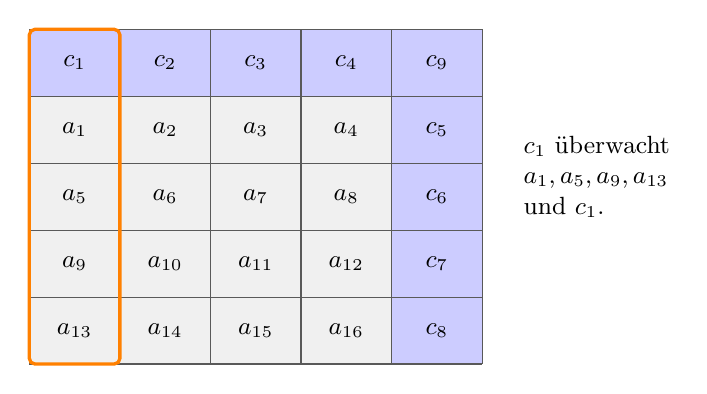
\begin{tikzpicture}[
            x=1.15cm,y=0.85cm,
            every node/.style={font=\small}
        ]
        % Nachrichtenbits
        \foreach \r in {1,...,4} {
                \foreach \c in {1,...,4} {
                        \pgfmathtruncatemacro{\nr}{4*(\r-1)+\c}
                        \fill[gray!12] (\c-1,-\r) rectangle (\c,-\r+1);
                        \node at (\c-.5,-\r+.5) {\(a_{\nr}\)};
                    }
            }

        % Kontrollbits der Spalten
        \foreach \c in {1,...,4} {
                \fill[blue!20] (\c-1,0) rectangle (\c,1);
                \node at (\c-.5,.5) {\(c_{\c}\)};
            }

        % Kontrollbits der Zeilen
        \foreach \r in {1,...,4} {
                \pgfmathtruncatemacro{\nr}{\r+4}
                \fill[blue!20] (4,-\r) rectangle (5,-\r+1);
                \node at (4.5,-\r+.5) {\(c_{\nr}\)};
            }

        % Kontrollbit oben rechts
        \fill[blue!20] (4,0) rectangle (5,1);
        \node at (4.5,.5) {\(c_9\)};

        % Gitter
        \draw[step=1,black!65] (0,-4) grid (5,1);

        % Beispiel: Überwachungsbereich von c1
        \draw[orange,very thick,rounded corners=2pt]
        (0,-4) rectangle (1,1);

        \node[anchor=west,align=left] at (5.35,-1.2)
        {\(c_1\) überwacht\\
            \(a_1,a_5,a_9,a_{13}\)\\
            und \(c_1\).};
    \end{tikzpicture}
\end{center}


Die Überwachungsbereiche lassen sich in einer sogenannten
\emph{Überwachungstabelle} darstellen. Jede Spalte entspricht
einem Bit des Codeworts und jede Zeile einem Kontrollbit.
Ein Kreuz in der Tabelle bedeutet, dass das entsprechende Bit
vom jeweiligen Kontrollbit überwacht wird.


\begin{center}
    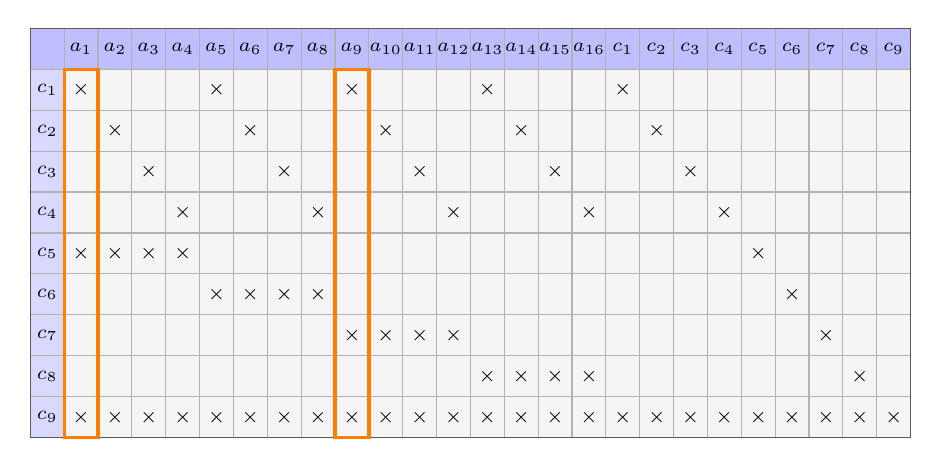
\begin{tikzpicture}[
            x=0.43cm,y=0.52cm,
            every node/.style={font=\scriptsize}
        ]
        % Tabellenhintergrund
        \fill[blue!25] (0,0) rectangle (26,1);
        \fill[blue!15] (0,-9) rectangle (1,0);
        \fill[gray!8] (1,-9) rectangle (26,0);

        % Spaltenbeschriftung
        \foreach \i in {1,...,16} {
                \pgfmathsetmacro{\xx}{\i+.5}
                \node at (\xx,.5) {\(a_{\i}\)};
            }
        \foreach \i in {1,...,9} {
                \pgfmathtruncatemacro{\col}{16+\i}
                \node at (\col+.5,.5) {\(c_{\i}\)};
            }

        % Zeilenbeschriftung
        \foreach \i in {1,...,9} {
                \node at (.5,.5-\i) {\(c_{\i}\)};
            }

        % Kontrollbits c1 bis c4 (Spalten)
        \foreach \j in {1,...,4} {
                \foreach \r in {0,...,3} {
                        \pgfmathtruncatemacro{\col}{\j+4*\r}
                        \node at (\col+.5,.5-\j) {\(\times\)};
                    }
            }

        % Kontrollbits c5 bis c8 (Zeilen)
        \foreach \r in {1,...,4} {
                \pgfmathtruncatemacro{\row}{\r+4}
                \foreach \j in {1,...,4} {
                        \pgfmathtruncatemacro{\col}{4*(\r-1)+\j}
                        \node at (\col+.5,.5-\row) {\(\times\)};
                    }
            }

        % Jedes Kontrollbit überwacht sich selbst
        \foreach \i in {1,...,8} {
                \pgfmathtruncatemacro{\col}{16+\i}
                \node at (\col+.5,.5-\i) {\(\times\)};
            }

        % c9 überwacht sämtliche Bits
        \foreach \col in {1,...,25} {
                \node at (\col+.5,-8.5) {\(\times\)};
            }

        % Gitter
        \draw[step=1,black!30,thin] (0,-9) grid (26,1);
        \draw[black!65] (0,-9) rectangle (26,1);

        % Hervorhebung der ersten Spalte
        \draw[orange,very thick]
        (1,-9) rectangle (2,0);

        % Hervorhebung der neunten Spalte
        \draw[orange,very thick]
        (9,-9) rectangle (10,0);
    \end{tikzpicture}
\end{center}


Tritt bei der Übertragung ein einzelner Bitfehler auf, so stimmen
die Paritätsbedingungen genau jener Kontrollbits nicht mehr,
die das fehlerhafte Bit überwachen. Beispielsweise wird ein Fehler
im Bit \(a_1\) von den Kontrollbits \(c_1,c_5\) und \(c_9\)
registriert. Ein Fehler im Bit \(a_9\) wird dagegen von
\(c_1,c_7\) und \(c_9\) registriert. (Markierte Spalten in der Überwachungstabelle.)

Die Kombination der Kontrollbits, die einen Fehler registrieren,
bildet somit eine Art \emph{Signatur des fehlerhaften Bits}.
Anhand dieser Signatur können wir bestimmen, welches Bit
umgeflippt wurde.

Damit dies eindeutig möglich ist, müssen die Spalten der
Überwachungstabelle paarweise verschieden sein. Ausserdem darf
keine Spalte ausschliesslich aus leeren Feldern bestehen, da
ein Fehler im entsprechenden Bit sonst von keinem Kontrollbit
erkannt würde.
\begin{myremark}
    Eine Kodierung ist genau dann 1-fehlerkorrigierend,
    wenn die Spalten ihrer Überwachungstabelle paarweise verschieden
    und keine davon leer ist.
\end{myremark}



\subsection*{Wie viele Kontrollbits sind mindestens notwendig?}

Betrachten wir nun eine Nachricht mit 16 Bit. Bei der
Kartentrick-Methode haben wir dafür neun Kontrollbits verwendet.
Allerdings zeigt die Überwachungstabelle, dass das neunte
Kontrollbit \(c_9\) überflüssig ist: Auch wenn wir auf dieses
Kontrollbit verzichten, bleiben alle Spalten paarweise
verschieden und nicht leer. Wir können also bereits mit
acht Kontrollbits sämtliche Einzelfehler korrigieren.

Doch wie viele Kontrollbits benötigen wir mindestens?

Mit \(n\) Kontrollbits besitzt die Überwachungstabelle \(n\) Zeilen.
In jeder Spalte kann ein Kreuz entweder vorhanden sein oder
fehlen. Somit gibt es insgesamt \(2^n\) verschiedene Möglichkeiten,
eine Spalte zu gestalten. Da eine Spalte ohne Kreuze nicht
verwendet werden darf, bleiben

\[
    2^n-1
\]

nutzbare Spalten.

Für eine Nachricht mit 16 Bit und \(n\) Kontrollbits benötigen
wir insgesamt \(16+n\) verschiedene Spalten. Deshalb muss gelten:

\[
    2^n-1\geq 16+n.
\]

Mit vier Kontrollbits erhalten wir höchstens
\(2^4-1=15\) nutzbare Spalten. Dies reicht nicht aus.
Mit fünf Kontrollbits stehen dagegen
\(2^5-1=31\) verschiedene Spalten zur Verfügung.
Das genügt für die insgesamt 21 Bits des Codeworts.

Für die 1-fehlerkorrigierende Kodierung einer Nachricht
mit 16 Bit sind somit mindestens fünf Kontrollbits notwendig.

\begin{myremark}
    Allgemein gilt für eine Nachricht der Länge \(m\), dass die
    minimale Anzahl \(n\) der Kontrollbits die folgende Ungleichung
    erfüllen muss:
    \[
        2^n-1\geq m+n
    \]
\end{myremark}





\subsection*{Konstruktion einer optimalen Überwachungstabelle}

Wir wissen nun, dass fünf Kontrollbits für eine Nachricht
mit 16 Bit ausreichen können. Wie lässt sich eine
entsprechende Kodierung konstruieren?

Dazu erstellen wir eine Überwachungstabelle mit fünf Zeilen
und 21 Spalten. Die ersten 16 Spalten entsprechen den
Nachrichtenbits \(a_1,\ldots,a_{16}\), die letzten fünf den
Kontrollbits \(c_1,\ldots,c_5\).

\begin{center}
    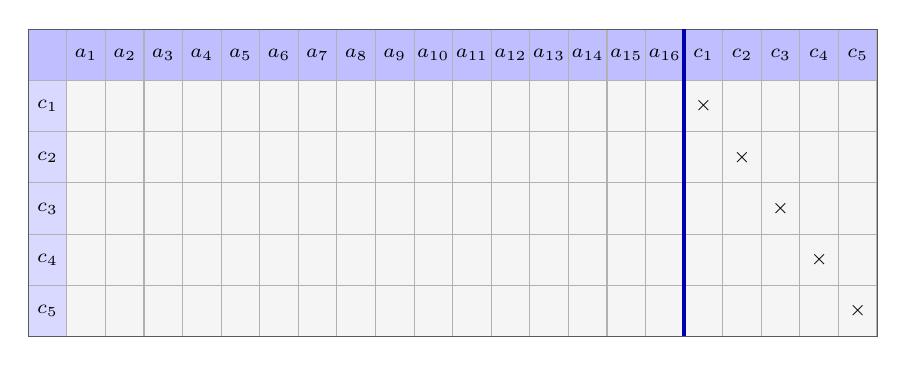
\begin{tikzpicture}[
            x=0.49cm,y=0.65cm,
            every node/.style={font=\scriptsize}
        ]
        % Hintergrund
        \fill[blue!25] (0,0) rectangle (22,1);
        \fill[blue!15] (0,-5) rectangle (1,0);
        \fill[gray!8] (1,-5) rectangle (22,0);

        % Spaltenbeschriftung
        \foreach \i in {1,...,16} {
                \node at (\i+.5,.5) {\(a_{\i}\)};
            }
        \foreach \i in {1,...,5} {
                \pgfmathtruncatemacro{\col}{16+\i}
                \node at (\col+.5,.5) {\(c_{\i}\)};
            }

        % Zeilenbeschriftung
        \foreach \i in {1,...,5} {
                \node at (.5,.5-\i) {\(c_{\i}\)};
            }

        % Kontrollbits: Einheitsmatrix
        \foreach \i in {1,...,5} {
                \pgfmathtruncatemacro{\col}{16+\i}
                \node at (\col+.5,.5-\i) {\(\times\)};
            }

        % Gitter
        \draw[step=1,black!30,thin] (0,-5) grid (22,1);
        \draw[black!65] (0,-5) rectangle (22,1);

        % Trennung Nachrichtenbits / Kontrollbits
        \draw[blue!70!black,very thick] (17,-5) -- (17,1);
    \end{tikzpicture}
\end{center}

Jedes Kontrollbit überwacht sich selbst. Daher tragen wir
in der Spalte von \(c_1\) ein Kreuz in der ersten Zeile ein,
in der Spalte von \(c_2\) eines in der zweiten Zeile usw.
Die übrigen Felder dieser fünf Spalten bleiben leer.

Die Einträge für die 16 Nachrichtenbits wählen wir
anschliessend so, dass alle Spalten paarweise verschieden
und nicht leer sind. Dabei gibt es verschiedene Möglichkeiten.
Jede solche Wahl führt zu einer 1-fehlerkorrigierenden
Kodierung mit fünf Kontrollbits.


\begin{center}
    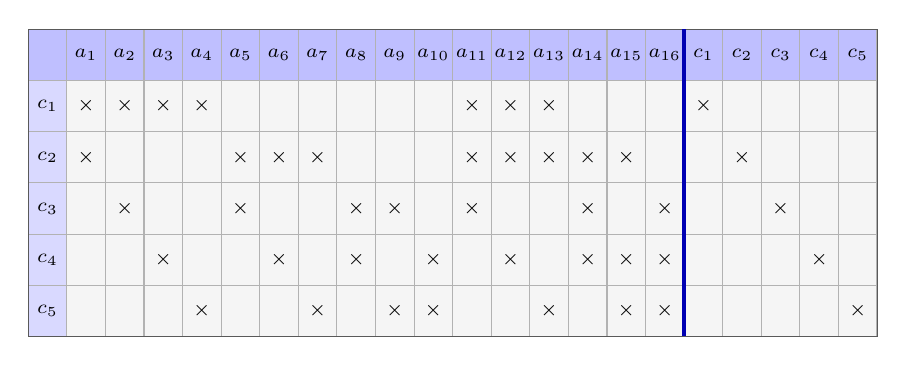
\begin{tikzpicture}[
            x=0.49cm,y=0.65cm,
            every node/.style={font=\scriptsize}
        ]
        % Hintergrund
        \fill[blue!25] (0,0) rectangle (22,1);
        \fill[blue!15] (0,-5) rectangle (1,0);
        \fill[gray!8] (1,-5) rectangle (22,0);

        % Spaltenbeschriftung
        \foreach \i in {1,...,16} {
                \node at (\i+.5,.5) {\(a_{\i}\)};
            }
        \foreach \i in {1,...,5} {
                \pgfmathtruncatemacro{\col}{16+\i}
                \node at (\col+.5,.5) {\(c_{\i}\)};
            }

        % Zeilenbeschriftung
        \foreach \i in {1,...,5} {
                \node at (.5,.5-\i) {\(c_{\i}\)};
            }

        % Überwachungsbereiche der Nachrichtenbits
        \foreach \col in {1,2,3,4,11,12,13} {
                \node at (\col+.5,-.5) {\(\times\)};
            }
        \foreach \col in {1,5,6,7,11,12,13,14,15} {
                \node at (\col+.5,-1.5) {\(\times\)};
            }
        \foreach \col in {2,5,8,9,11,14,16} {
                \node at (\col+.5,-2.5) {\(\times\)};
            }
        \foreach \col in {3,6,8,10,12,14,15,16} {
                \node at (\col+.5,-3.5) {\(\times\)};
            }
        \foreach \col in {4,7,9,10,13,15,16} {
                \node at (\col+.5,-4.5) {\(\times\)};
            }

        % Kontrollbits: Einheitsmatrix
        \foreach \i in {1,...,5} {
                \pgfmathtruncatemacro{\col}{16+\i}
                \node at (\col+.5,.5-\i) {\(\times\)};
            }

        % Gitter
        \draw[step=1,black!30,thin] (0,-5) grid (22,1);
        \draw[black!65] (0,-5) rectangle (22,1);

        % Trennung Nachrichtenbits / Kontrollbits
        \draw[blue!70!black,very thick] (17,-5) -- (17,1);
    \end{tikzpicture}
\end{center}


Um eine Nachricht zu kodieren, bestimmen wir die Kontrollbits
nacheinander. Dabei betrachten wir jeweils diejenigen
Nachrichtenbits, die vom entsprechenden Kontrollbit überwacht
werden. Das Kontrollbit wird so gewählt, dass die Gesamtzahl
der Einsen gerade ist.

\begin{myexample}
    Die Nachricht

    \[
        \texttt{0101 1111 0010 1011}
    \]

    soll mit der Überwachungstabelle oben durch Kontrollbits ergänzt werden.

    Das Kontrollbit \(c_1\) überwacht die Nachrichtenbits \(a_1, a_2, a_3, a_4, a_{11}, a_{12}\) und \(a_{13}\).
    \[
        \texttt{\textcolor{orange}{0101} 1111 00\textcolor{orange}{10 1}011}
    \]
    Die Anzahl Einser in den überwachten Nachrichtenbits ist gerade, also \(c_1 = 0\).


    Das Kontrollbit \(c_2\) überwacht die Nachrichtenbits \(a_1, a_5, a_6, a_7, a_{11}, a_{12}, a_{13}, a_{14}\) und \(a_{15}\).
    \[
        \texttt{\textcolor{orange}{0}101 \textcolor{orange}{111}1 00\textcolor{orange}{10 101}1}
    \]
    Die Anzahl Einser in den überwachten Nachrichtenbits ist gerade, also \(c_2 = 0\).

    usw.

    Schliesslich erhalten wir mit der Überwachungstabelle oben
    die Kontrollbits

    \[
        \texttt{00101}.
    \]

    Das vollständige Codewort lautet damit

    \[
        \underbrace{\texttt{0101 1111 0010 1011}}_{\text{Nachricht}}
        \ \underbrace{\texttt{00101}}_{\text{Kontrollbits}}.
    \]

    Bei der Übertragung eines solchen Codeworts kann ein einzelner
    Bitfehler anhand der verletzten Paritätsbedingungen eindeutig
    lokalisiert und anschliessend korrigiert werden.
\end{myexample}


\begin{myexercise}



    Arbeiten Sie für die folgenden Fragen mit dieser
    Überwachungstabelle:

    \begin{center}
        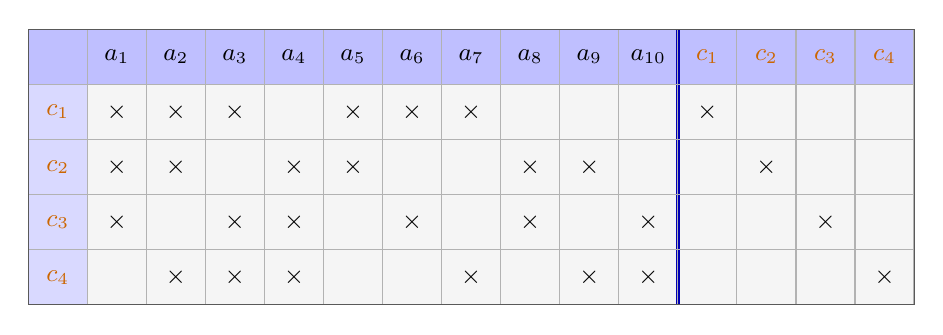
\begin{tikzpicture}[
                x=0.75cm,
                y=0.7cm,
                every node/.style={font=\small}
            ]

            % Hintergrund
            \fill[blue!25] (0,0) rectangle (15,1);
            \fill[blue!15] (0,-4) rectangle (1,0);
            \fill[gray!8] (1,-4) rectangle (15,0);


            % Spaltenbeschriftungen: Nachrichtenbits
            \foreach \i in {1,...,10} {
                    \node at (\i+0.5,0.5) {\(a_{\i}\)};
                }

            % Spaltenbeschriftungen: Kontrollbits
            \foreach \i in {1,...,4} {
                    \pgfmathtruncatemacro{\col}{10+\i}
                    \node[text=orange!80!black]
                    at (\col+0.5,0.5) {\(c_{\i}\)};
                }

            % Zeilenbeschriftungen
            \foreach \i in {1,...,4} {
                    \node[text=orange!80!black]
                    at (0.5,0.5-\i) {\(c_{\i}\)};
                }

            % Überwachungsbereich c1
            \foreach \col in {1,2,3,5,6,7,11} {
                    \node at (\col+0.5,-0.5) {\(\times\)};
                }

            % Überwachungsbereich c2
            \foreach \col in {1,2,4,5,8,9,12} {
                    \node at (\col+0.5,-1.5) {\(\times\)};
                }

            % Überwachungsbereich c3
            \foreach \col in {1,3,4,6,8,10,13} {
                    \node at (\col+0.5,-2.5) {\(\times\)};
                }

            % Überwachungsbereich c4
            \foreach \col in {2,3,4,7,9,10,14} {
                    \node at (\col+0.5,-3.5) {\(\times\)};
                }



            % Trennung Nachrichtenbits / Kontrollbits
            \draw[blue!70!black,very thick] (11,-4) -- (11,1);

            % Gitter
            \draw[step=1,black!30,thin]
            (0,-4) grid (15,1);

            % Äusserer Rahmen
            \draw[black!65]
            (0,-4) rectangle (15,1);

        \end{tikzpicture}
    \end{center}

    \begin{enumerate}
        \item Alice möchte die Nachricht
              \texttt{0101 0101 01} versenden.
              Wie lautet die Nachricht samt Kontrollbits?

        \item Bob erhält die Nachricht
              \texttt{1111 1111 11}
              \textcolor{magenta}{\texttt{1001}}.
              Wie lautet die ursprüngliche Nachricht,
              wenn man davon ausgeht, dass bei der
              Übermittlung höchstens ein Fehler
              passiert ist?

        \item Cedric erhält die Nachricht
              \texttt{1010 1010 11}
              \textcolor{magenta}{\texttt{0111}}.
              Wo ist der Fehler passiert?
    \end{enumerate}

    \begin{myanswer}
        \begin{enumerate}
            \item Die von Alice versendete Nachricht lautet:
                  \[
                      \texttt{0101 0101 01}\,
                      \textcolor{orange}{\texttt{0101}}
                  \]

            \item Die von Bob erhaltene Nachricht hat einen Fehler
                  beim Bit \(a_7\). Ursprünglich lautete die Nachricht:
                  \[
                      \texttt{1111 1101 11}
                  \]

            \item Bei der Nachricht, die Cedric erhält, ist der Fehler
                  im letzten Kontrollbit \(c_4\) passiert.
                  Das korrekte Codewort lautet:
                  \[
                      \texttt{1010 1010 11}\,
                      \textcolor{orange}{\texttt{0110}}
                  \]
        \end{enumerate}
    \end{myanswer}

\end{myexercise}



\begin{myexercise}
    Alice möchte eine 1-fehlerkorrigierende Kodierung für
    8 verschiedene Nachrichten entwerfen. Für die Kodierung
    dieser Nachrichten (ohne Kontrollbits) verwendet sie
    Bitfolgen der Länge 3
    (\texttt{000}, \texttt{001}, \ldots, \texttt{111}).

    \begin{enumerate}
        \item Wie viele Kontrollbits sind für eine
              1-fehlerkorrigierende Kodierung mindestens notwendig?

        \item Entwerfen Sie eine solche Kodierung, indem Sie
              die entsprechende Überwachungstabelle angeben.
    \end{enumerate}
    \begin{myanswer}

        Die Anzahl \(n\) der Kontrollbits muss so gross sein, dass
        \[
            2^n-1 \geq 3+n
        \]
        gilt. Daraus folgt \(n\geq 3\). Es werden also mindestens
        drei Kontrollbits benötigt.

        Eine mögliche Überwachungstabelle ist:

        \begin{center}
            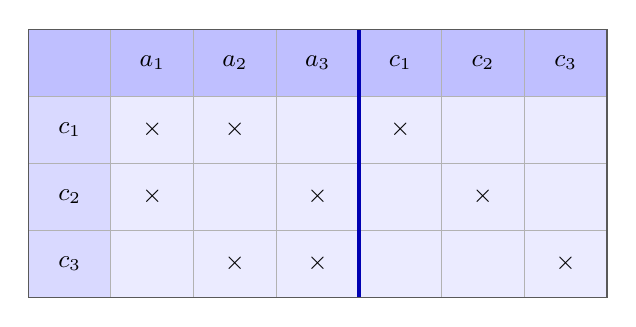
\begin{tikzpicture}[
                    x=1.05cm,
                    y=0.85cm,
                    every node/.style={font=\small}
                ]


                % Hintergrund
                \fill[blue!25] (0,0) rectangle (7,1);
                \fill[blue!15] (0,-3) rectangle (1,0);
                \fill[blue!8] (1,-3) rectangle (7,0);

                % Spaltenbeschriftungen
                \foreach \i in {1,...,3} {
                        \node at (\i+0.5,0.5) {\(a_{\i}\)};
                    }
                \foreach \i in {1,...,3} {
                        \pgfmathtruncatemacro{\col}{3+\i}
                        \node at (\col+0.5,0.5) {\(c_{\i}\)};
                    }

                % Zeilenbeschriftungen
                \foreach \i in {1,...,3} {
                        \node at (0.5,0.5-\i) {\(c_{\i}\)};
                    }

                % Überwachungsbereich c1
                \foreach \col in {1,2,4} {
                        \node at (\col+0.5,-0.5) {\(\times\)};
                    }

                % Überwachungsbereich c2
                \foreach \col in {1,3,5} {
                        \node at (\col+0.5,-1.5) {\(\times\)};
                    }

                % Überwachungsbereich c3
                \foreach \col in {2,3,6} {
                        \node at (\col+0.5,-2.5) {\(\times\)};
                    }

                % Gitter
                \draw[step=1,black!30,thin] (0,-3) grid (7,1);

                % Trennung Nachrichtenbits / Kontrollbits
                \draw[blue!70!black,very thick] (4,-3) -- (4,1);


                % Äusserer Rahmen
                \draw[black!65]
                (0,-3) rectangle (7,1);

            \end{tikzpicture}
        \end{center}

        Die Spalten der Überwachungstabelle sind paarweise verschieden
        und keine Spalte ist leer. Damit kann jeder einzelne Bitfehler
        eindeutig lokalisiert und korrigiert werden.

    \end{myanswer}
\end{myexercise}


\begin{myexercise}
    Bob benötigt eine 1-fehlerkorrigierende Kodierung
    für eine Million verschiedene Nachrichten.

    \begin{enumerate}
        \item Wie viele Bits sind für die Kodierung der
              Nachrichten nötig (ohne Kontrollbits)?

        \item Wie viele Kontrollbits werden mindestens benötigt?
    \end{enumerate}
    \begin{myanswer}
        Für eine Million verschiedene Nachrichten sind Bitfolgen der
        Länge 20 nötig, denn es gilt
        \[
            2^{19} < 10^6 < 2^{20}.
        \]

        Die Anzahl \(n\) der Kontrollbits muss so gross sein, dass
        \[
            2^n-1 \geq 20+n
        \]
        gilt. Für \(n=4\) ist diese Bedingung nicht erfüllt, für
        \(n=5\) hingegen schon:
        \[
            2^5-1=31\geq 25.
        \]

        Es werden also mindestens \textbf{5 Kontrollbits} benötigt.
    \end{myanswer}
\end{myexercise}


\begin{myexercise}

    Entwerfen Sie eine 1-fehlerkorrigierende Kodierung für
    30 verschiedene Nachrichten. Geben Sie die entsprechende
    Überwachungstabelle an.
    \begin{myanswer}

        Für 30 verschiedene Nachrichten benötigt man Bitfolgen der Länge 5,
        da \(2^4 < 30 \leq 2^5\) gilt.

        Für die Anzahl \(n\) der Kontrollbits muss gelten:
        \[
            2^n-1 \geq 5+n.
        \]
        Daraus folgt \(n\geq 4\). Es werden also mindestens
        vier Kontrollbits benötigt.

        Eine mögliche Überwachungstabelle ist:

        \begin{center}
            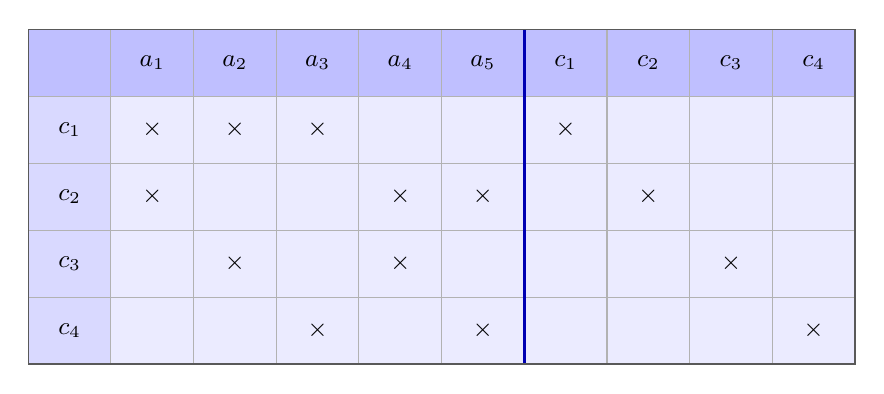
\begin{tikzpicture}[
                    x=1.05cm,
                    y=0.85cm,
                    every node/.style={font=\small}
                ]


                % Hintergrund
                \fill[blue!25] (0,0) rectangle (10,1);
                \fill[blue!15] (0,-4) rectangle (1,0);
                \fill[blue!8] (1,-4) rectangle (10,0);

                % Spaltenbeschriftungen: Nachrichtenbits
                \foreach \i in {1,...,5} {
                        \node at (\i+0.5,0.5) {\(a_{\i}\)};
                    }

                % Spaltenbeschriftungen: Kontrollbits
                \foreach \i in {1,...,4} {
                        \pgfmathtruncatemacro{\col}{5+\i}
                        \node at (\col+0.5,0.5) {\(c_{\i}\)};
                    }

                % Zeilenbeschriftungen
                \foreach \i in {1,...,4} {
                        \node at (0.5,0.5-\i) {\(c_{\i}\)};
                    }

                % Überwachungsbereich c1
                \foreach \col in {1,2,3,6} {
                        \node at (\col+0.5,-0.5) {\(\times\)};
                    }

                % Überwachungsbereich c2
                \foreach \col in {1,4,5,7} {
                        \node at (\col+0.5,-1.5) {\(\times\)};
                    }

                % Überwachungsbereich c3
                \foreach \col in {2,4,8} {
                        \node at (\col+0.5,-2.5) {\(\times\)};
                    }

                % Überwachungsbereich c4
                \foreach \col in {3,5,9} {
                        \node at (\col+0.5,-3.5) {\(\times\)};
                    }

                % Gitter
                \draw[step=1,black!30,thin] (0,-4) grid (10,1);

                % Trennung Nachrichtenbits / Kontrollbits
                \draw[blue!70!black,very thick] (6,-4) -- (6,1);


                % Äusserer Rahmen
                \draw[black!65]
                (0,-4) rectangle (10,1);


            \end{tikzpicture}
        \end{center}

        Da alle Spalten der Überwachungstabelle paarweise verschieden
        und nicht leer sind, kann jeder einzelne Bitfehler eindeutig
        lokalisiert und korrigiert werden.

    \end{myanswer}
\end{myexercise}










\subsection*{Historischer Hintergrund: Richard Hamming}

Die Entwicklung effizienter fehlerkorrigierender Codes ist
eng mit dem amerikanischen Mathematiker Richard Hamming
(1915--1998) verbunden.

Hamming arbeitete zunächst am Manhattan-Projekt und später
bei den Bell Laboratories. Zu dieser Zeit wurden Programme
und Daten unter anderem mithilfe von Lochkarten gespeichert
und eingegeben. Ein Loch entsprach dabei einer 1, eine Stelle
ohne Loch einer 0.

\begin{figure}[H]
    \centering
    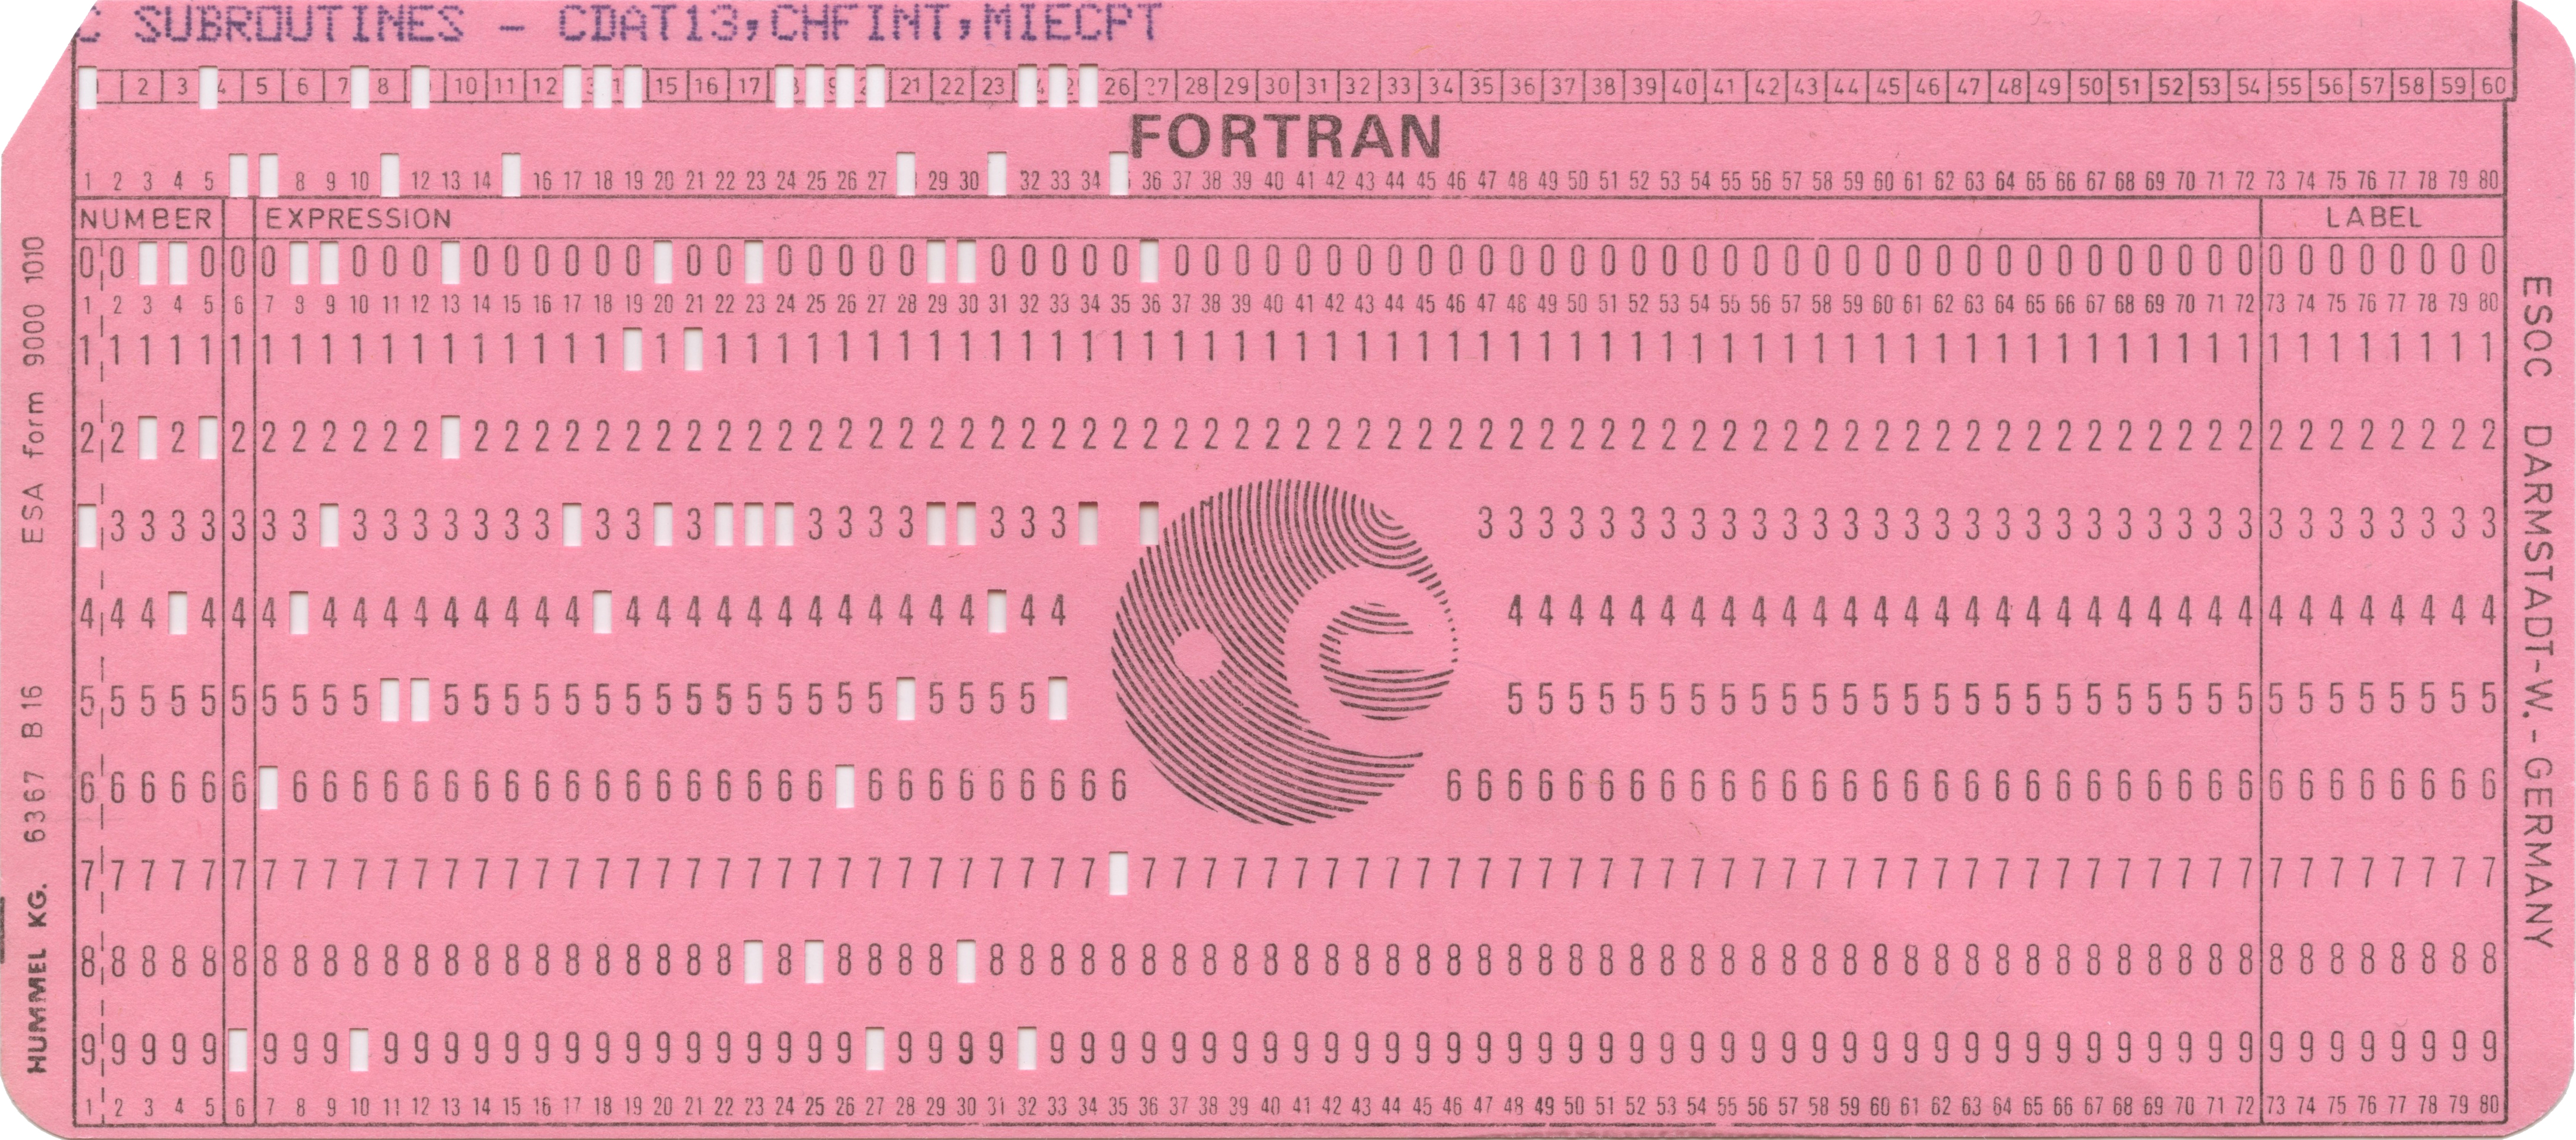
\includegraphics[width = 0.5\textwidth]{Grundlagen_Info/05_Datenintegritaet/Figures/Fortran_punch_card_ESA.jpg}
    \caption[Fortran Lochkarte der European Space Agency (ESA), 70er Jahre]{Fortran Lochkarte der European Space Agency (ESA), 70er Jahre, Till Niermann, CC BY-SA 3.0, via \href{https://commons.wikimedia.org/wiki/File:Fortran_punch_card_ESA.jpg}{Wikimedia Commons}}
    \label{fig:lochkarte}
\end{figure}

Fehler beim Erstellen oder Lesen der Lochkarten konnten dazu
führen, dass Programme nicht korrekt ausgeführt wurden.
Besonders ärgerlich war, dass solche Fehler oft erst nach
längerer Rechenzeit bemerkt wurden.

Hamming beschäftigte sich deshalb mit der Frage, wie sich
solche Fehler automatisch erkennen und korrigieren lassen.
Daraus entstanden die nach ihm benannten \emph{Hamming-Codes},
die mit vergleichsweise wenigen Kontrollbits einzelne
Bitfehler korrigieren können.

Die Grundidee entspricht dem Verfahren, das wir gerade
untersucht haben: Jedes Bit wird durch eine bestimmte
Kombination von Kontrollbits überwacht. Aus den verletzten
Paritätsbedingungen lässt sich die Position eines einzelnen
fehlerhaften Bits bestimmen.

Damit bilden die Hamming-Codes eine wichtige Grundlage
der Fehlerkorrektur in digitalen Informationssystemen.

\begin{myexercise}
    Mit unseren Überlegungen konnten wir die minimale Anzahl
    Kontrollbits für eine 1-fehler-korrigierende Kodierung ermitteln.
    Bei der Erstellung der entsprechenden Überwachungstabellen
    haben wir viele Freiheiten. Entscheidend ist lediglich, dass
    alle Spalten paarweise verschieden sind und keine Spalte leer ist.

    Richard Hamming entwickelte eine elegante Methode, mit der
    sich systematisch festlegen lässt, welche Bits von den einzelnen
    Kontrollbits überwacht werden und an welchen Positionen die
    Kontrollbits innerhalb des Codeworts stehen sollen. Schliesslich
    müssen die Kontrollbits nicht zwingend am Ende der Nachricht
    angefügt werden.

    Weitere Informationen zur Funktionsweise der Hamming-Codes
    finden Sie im folgenden Video:

    \begin{center}
        \url{https://www.youtube.com/watch?v=X8jsijhllIA}
    \end{center}



    \begin{enumerate}
        \item Alice möchte den erweiterten \((16,11)\)-Hamming-Code verwenden,
              um die Nachricht \texttt{1011 1100 010} zu versenden.
              Wie lautet die um die Kontrollbits ergänzte Nachricht?

        \item Bob erhält die mit dem erweiterten \((16,11)\)-Hamming-Code
              kodierte Nachricht \texttt{0001 1011 0010 0011}.
              Korrigieren Sie den Fehler in der Nachricht.
    \end{enumerate}

    \begin{myanswer}

        \begin{enumerate}
            \item Die von Alice versendete Nachricht lautet:
                  \[
                      \texttt{0111 1011 1110 0010}
                  \]

                  \begin{center}
                      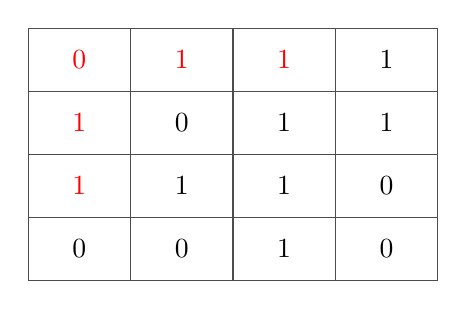
\begin{tikzpicture}[
                              x=1.3cm, y=0.8cm,
                              every node/.style={font=\normalsize}
                          ]
                          \foreach \row/\col/\bit in {
                                  1/1/0, 1/2/1, 1/3/1, 1/4/1,
                                  2/1/1, 2/2/0, 2/3/1, 2/4/1,
                                  3/1/1, 3/2/1, 3/3/1, 3/4/0,
                                  4/1/0, 4/2/0, 4/3/1, 4/4/0
                              } {
                                  \node at (\col-.5,4.5-\row) {\bit};
                              }

                          % Kontrollbits rot hervorheben
                          \foreach \col/\row/\bit in {
                                  1/1/0, 2/1/1, 3/1/1,
                                  1/2/1, 1/3/1
                              } {
                                  \node[red,fill=white,inner sep=1pt]
                                  at (\col-.5,4.5-\row) {\bit};
                              }

                          \draw[step=1,black!70] (0,0) grid (4,4);
                      \end{tikzpicture}
                  \end{center}

            \item Die von Bob erhaltene Nachricht enthält einen
                  Fehler an der Position 13 (Positionen ab 0 gezählt,
                  also beim 14.\ Bit). Das entsprechende Bit
                  muss von 0 auf 1 korrigiert werden.

                  \begin{center}
                      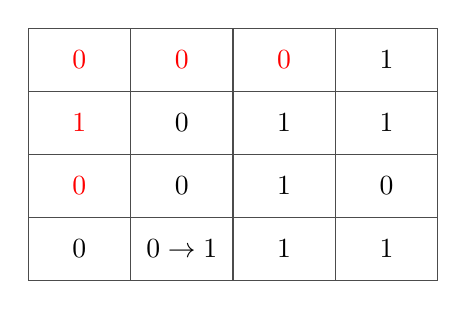
\begin{tikzpicture}[
                              x=1.3cm, y=0.8cm,
                              every node/.style={font=\normalsize}
                          ]
                          \foreach \row/\col/\bit in {
                                  1/1/0, 1/2/0, 1/3/0, 1/4/1,
                                  2/1/1, 2/2/0, 2/3/1, 2/4/1,
                                  3/1/0, 3/2/0, 3/3/1, 3/4/0,
                                  4/1/0, 4/2/0, 4/3/1, 4/4/1
                              } {
                                  \node at (\col-.5,4.5-\row) {\bit};
                              }
                          % Kontrollbits rot hervorheben
                          \foreach \col/\row/\bit in {
                                  1/1/0, 2/1/0, 3/1/0,
                                  1/2/1, 1/3/0
                              } {
                                  \node[red,fill=white,inner sep=1pt]
                                  at (\col-.5,4.5-\row) {\bit};
                              }

                          % Fehlerkorrektur an Position 13
                          \node[fill=white,inner sep=1pt]
                          at (1.5,.5)
                          {\(\cancel{0}\rightarrow 1\)};

                          \draw[step=1,black!70] (0,0) grid (4,4);
                      \end{tikzpicture}
                  \end{center}
        \end{enumerate}

    \end{myanswer}

\end{myexercise}

\section{Der \glsentryshort{XOR}-Operator}

Um das Paritätsbit zweier binärer Codes zu berechnen, wird der \textbf{\acrshort{XOR}-Operator} (\enquote{Exklusives Oder}, $\oplus$) verwendet. Die Addition modulo 2 zweier Bits (\acrshort{XOR}) ist definiert in \cref{tab:mod2}.

\begin{table}[H]
    \centering
    \begin{tabular}{ccc}
        A & B & A $\oplus$ B \\\midrule
        0 & 0 & 0            \\\midrule
        0 & 1 & 1            \\\midrule
        1 & 0 & 1            \\\midrule
        1 & 1 & 0            \\
    \end{tabular}
    \caption{\glsentryshort{XOR} (Addition modulo 2) für alle 4 möglichen Bit-Kombinationen}
    \label{tab:mod2}
\end{table}

Das Ergebnis ist also genau dann 1, wenn genau eines der beiden Eingangsbits gleich 1 ist. \acrshort{XOR} wird auch \enquote{Addition modulo 2} genannt, da das Resultat einer \acrshort{XOR}-Operation immer genau der Summe beider Bits modulo 2 entspricht.

\acrshort{XOR} kann nicht nur auf einzelne Bits, sondern auch auf mehrere Bitfolgen angewendet werden. Dabei wird jedes Bit der Folge 1 mit dem Bit der Folge 2 an derselben Stelle verglichen. Das Resultat einer \acrshort{XOR}-Operation wird Parität ($P$) genannt.


\begin{myexample}
Gegeben seien drei Datenblöcke:

\[
    D_1 = 1011_2, \quad D_2 = 1100_2, \quad D_3 = 0110_2
\]

Die Parität \( P \) wird durch \acrshort{XOR}-Verknüpfung berechnet:

\[
    P = D_1 \oplus D_2 \oplus D_3
\]

Wir berechnen schrittweise:

\[
    D_1 \oplus D_2 = 1011_2 \oplus 1100_2 = 0111_2
\]

\[
    P = 0111_2 \oplus 0110_2 = 0001_2
\]

Das Paritätsbit wird zusammen mit den Daten gespeichert. Fällt eine Festplatte aus, kann der fehlende Wert durch Umstellen der \acrshort{XOR}-Operation wiederhergestellt werden.
\end{myexample}


\begin{myexercise}
    Gegeben sind die folgenden binären Codes:

    \[
        A = 1101_2, \quad B = 1010_2
    \]

    Berechnen Sie \( A \oplus B \).

    \begin{myanswer}
        Die Berechnung des \acrshort{XOR}-Operators erfolgt bitweise:

        \[
            A \oplus B = 1101_2 \oplus 1010_2
        \]

        Wir berechnen \acrshort{XOR} für jedes Bitpaar:

        \[
            \begin{array}{ccc}
                A & B & A \oplus B \\\midrule
                1 & 1 & 0          \\
                1 & 0 & 1          \\
                0 & 1 & 1          \\
                1 & 0 & 1          \\
            \end{array}
        \]

        Das ergibt:

        \[
            A \oplus B = 0111_2
        \]

        \textbf{Erklärung}:
        Der \acrshort{XOR}-Operator liefert 1, wenn die Eingangsbits unterschiedlich sind, und 0, wenn sie gleich sind. Da \( A \) und \( B \) an den Positionen 2, 3 und 4 unterschiedlich sind, stehen dort Einsen im Ergebnis.

    \end{myanswer}
\end{myexercise}


\begin{myexercise}
    Gegeben sind vier binäre Codes:

    \[
        A = 1011_2, \quad B = 1100_2, \quad C = 0110_2, \quad D = 1001_2
    \]

    Berechnen Sie \( A \oplus B \oplus C \oplus D \).

    \begin{myanswer}
        Die \acrshort{XOR}-Berechnung erfolgt schrittweise:

        \[
            A \oplus B = 1011_2 \oplus 1100_2
        \]

        Bitweise Berechnung:

        \[
            \begin{array}{ccc}
                A & B & A \oplus B \\\midrule
                1 & 1 & 0          \\
                0 & 1 & 1          \\
                1 & 0 & 1          \\
                1 & 0 & 1          \\
            \end{array}
        \]

        Das ergibt:

        \[
            A \oplus B = 0111_2
        \]

        Nun \acrshort{XOR} mit \( C \):

        \[
            0111_2 \oplus 0110_2
        \]

        \[
            0111_2 \oplus 0110_2 = 0001_2
        \]

        Danach \acrshort{XOR} mit \( D \):

        \[
            0001_2 \oplus 1001_2
        \]

        \[
            0001_2 \oplus 1001_2 = 1000_2
        \]

        Das Endergebnis lautet:

        \[
            A \oplus B \oplus C \oplus D = 1000_2
        \]

    \end{myanswer}
\end{myexercise}


\section{\glsentryshort{RAID}}

\gls{RAID} ist eine spannende Technologie, um die Funktionsweise von Paritätsbits in der Praxis zu illustrieren. \gls{RAID} ist ein Standard zur Organisation mehrerer Festplatten zu einem sogenannten logischen Laufwerk. Dabei werden mehrere physische Festplatten zu einer \enquote{virtuellen} Festplatte zusammengefasst. Ziel ist es, die Datensicherheit, die Ausfallsicherheit und/oder die Lese- und Schreib-Leistung zu verbessern. \gls{RAID} wird häufig in Servern und Speichersystemen eingesetzt, um Redundanz zu gewährleisten oder die Geschwindigkeit von Speicherzugriffen zu erhöhen.

Im Kontext der fehlerkorrigierenden und fehlererkennenden Kodierung spielt \gls{RAID} eine wichtige Rolle. Während \gls{RAID} 0 sich auf Performance ohne Redundanz konzentriert, nutzen andere \acrshort{RAID}-Level, insbesondere \gls{RAID} 5 und \gls{RAID} 6, Paritätsdaten zur Fehlerkorrektur. Im Folgenden schauen wir uns nur diejenigen \acrshort{RAID}-Typen an, welche heute am weitesten verbreitet sind.



\subsection{\glsentryshort{RAID} 0: Striping}
\gls{RAID} 0 verteilt Daten in Blöcken auf mehrere Festplatten (\textit{striping}), um die Lese- und Schreibgeschwindigkeit zu erhöhen. Dabei gibt es keine Redundanz, sodass der Ausfall einer einzigen Festplatte zu einem vollständigen Datenverlust führt.

\begin{itemize}
    \item Vorteil: Sehr hohe Geschwindigkeit bei Lese- und Schreiboperationen.
    \item Nachteil: Keine Fehlerkorrektur oder Redundanz; hoher Datenverlust bei Festplattendefekt.
\end{itemize}

\begin{figure}[H]
    \centering
    \includegraphics[width=0.25\linewidth]{Grundlagen_Info/05_Datenintegritaet/Figures/RAID_0}
    \caption[\glsentryshort{RAID}-0-Architektur mit zwei physischen Festplatten]{\glsentryshort{RAID}-0-Architektur mit zwei physischen Festplatten (Grafik: Cburnett, \href{https://commons.wikimedia.org/wiki/File:RAID_0.svg}{Wikimedia Commons}, CC BY-SA 3.0)}
    \label{fig:raid0}
\end{figure}

\begin{myexercise}
    Ein System verwendet \gls{RAID} 0 mit zwei Festplatten, wobei die Daten in 4-Byte-Blöcken verteilt werden. Gegeben ist die folgende Datei:

    \begin{verbatim}
ABCDEFGH
\end{verbatim}

    Wie werden die Daten auf den beiden Festplatten gespeichert?

    \begin{myanswer}
        \gls{RAID} 0 nutzt Striping ohne Redundanz. Die Daten werden in Blöcken zu je 4 Byte abwechselnd auf die beiden Festplatten geschrieben:

        \begin{verbatim}
Festplatte 1: ABCD
Festplatte 2: EFGH
\end{verbatim}

        Dieses Verfahren erhöht die Geschwindigkeit, bietet jedoch keine Ausfallsicherheit.
    \end{myanswer}
\end{myexercise}

\subsection{\glsentryshort{RAID} 1: Mirroring}
\gls{RAID} 1 speichert identische Kopien der Daten auf zwei Festplatten (\textit{mirroring}). Fällt eine Festplatte aus, können die Daten von der zweiten Festplatte wiederhergestellt werden.

\begin{itemize}
    \item Vorteil: Sehr hohe Datensicherheit, da jede Information doppelt gespeichert wird.
    \item Nachteil: Speicherplatz wird ineffizient genutzt, da nur die Hälfte der Gesamtkapazität verfügbar ist.
\end{itemize}

\begin{figure}[H]
    \centering
    \includegraphics[width=0.25\linewidth]{Grundlagen_Info/05_Datenintegritaet/Figures/RAID_1}
    \caption[\glsentryshort{RAID}-1-Architektur mit zwei physischen Festplatten]{\glsentryshort{RAID}-1-Architektur mit zwei physischen Festplatten (Grafik: Cburnett, \href{https://commons.wikimedia.org/wiki/File:RAID_1.svg}{Wikimedia Commons}, CC BY-SA 3.0)}
    \label{fig:raid1}
\end{figure}

Absicherung gegen Datenverlust kann mit lediglich 2 Festplatten nicht Speicherplatz-effizienter als mit \gls{RAID} 1 erfolgen, d.h., ein Verlust von 50\% des physischen Speicherplatzes muss in Kauf genommen werden. Effizientere Lösungen bieten sich an, wenn weitere Speicherplatten vorhanden sind. Selbstverständlich kann \gls{RAID} 1 auch mit 4, 6, 8 oder mehr Festplatten umgesetzt werden. Dabei bilden jeweils zwei Festplatten ein Spiegelpaar: Nutzbar bleibt die Hälfte der Gesamtkapazität, und pro Spiegelpaar darf eine Festplatte ausfallen. Fallen beide Festplatten desselben Paars aus, gehen Daten verloren.

\begin{myexercise}
    Ein Server verwendet \gls{RAID} 1 mit zwei Festplatten. Was passiert, wenn eine der beiden Festplatten ausfällt? Kann das System weiterhin genutzt werden?

    \begin{myanswer}
        \gls{RAID} 1 speichert eine vollständige Kopie aller Daten auf beiden Festplatten (Mirroring). Wenn eine Festplatte ausfällt, kann das System weiterhin auf die zweite Festplatte zugreifen, sodass keine Daten verloren gehen. Die ausgefallene Festplatte sollte jedoch ersetzt werden, um die Redundanz wiederherzustellen.
    \end{myanswer}
\end{myexercise}

\subsection{\glsentryshort{RAID} 4: Paritätsbits}
\gls{RAID} 4, 5 und 6 nutzen für die Datensicherheit statt \textit{mirroring} (Spiegelung der Daten) einen effizienteren Ansatz, um Daten über mehrere Laufwerke zu verteilen, indem sie Paritätsbits verwenden. Bei \gls{RAID} 4 werden die Daten wie bei \gls{RAID} 0 blockweise auf mehrere Festplatten verteilt. Zusätzlich gibt es eine eigene Paritäts-Festplatte, die für jeden \enquote{Striping-Block} $A_1A_2A_3\cdots$ genau ein Paritätsbit $A_p$ speichert (\cref{fig:raid4}).

\begin{figure}[H]
    \centering
    \includegraphics[width=0.45\linewidth]{Grundlagen_Info/05_Datenintegritaet/Figures/RAID_4}
    \caption[\glsentryshort{RAID}-4-Architektur mit vier physischen Festplatten und einem Paritätsbit]{\glsentryshort{RAID}-4-Architektur mit vier physischen Festplatten und einem Paritätsbit (Grafik: Cburnett, \href{https://commons.wikimedia.org/wiki/File:RAID_4.svg}{Wikimedia Commons}, CC BY-SA 3.0)}
    \label{fig:raid4}
\end{figure}

\subsection{\glsentryshort{RAID} 5: Verteilte Paritätsbits}
Da das Paritätsbit bei jedem Schreibvorgang neu geschrieben werden muss (auch bei kleinen Dateien), wird bei \gls{RAID} 4 die Paritäts-Festplatte übermässig stark beansprucht. Daher werden die Paritätsbits bei \gls{RAID} 5 im Gegensatz zu \gls{RAID} 4 auf alle Festplatten verteilt. Ansonsten funktioniert \gls{RAID} 5 identisch wie \gls{RAID} 4 (siehe \cref{fig:raid5}).


\begin{figure}[H]
    \centering
    \includegraphics[width=0.45\linewidth]{Grundlagen_Info/05_Datenintegritaet/Figures/RAID_5}
    \caption[\glsentryshort{RAID}-5-Architektur mit vier physischen Festplatten und einem \textit{verteilten} Paritätsbit]{\glsentryshort{RAID}-5-Architektur mit vier physischen Festplatten und einem \textit{verteilten} Paritätsbit (Grafik: Cburnett, \href{https://commons.wikimedia.org/wiki/File:RAID_5.svg}{Wikimedia Commons}, CC BY-SA 3.0)}
    \label{fig:raid5}
\end{figure}


Falls nun eine Festplatte ausfällt, können die verlorengegangenen Daten einfach rekonstruiert werden, indem das \textit{parity bit} über die verbliebenen Datenblöcke erneut berechnet wird. Somit ist ein Speicher-System bei \gls{RAID} 5 gegen den Ausfall einer Festplatte gesichert.

Bei \gls{RAID} 5 ist das Paritätsbit für jeden Block auf einer anderen Festplatte gespeichert, wodurch die Performance beim Schreiben von Daten erhöht wird, da die Schreib-Last so auf alle Festplatten gleichmässig verteilt werden kann.

Im Folgenden wird aufgezeigt, wie diese berechnet werden.

\gls{RAID} 5 verteilt die Paritätsinformationen über alle Festplatten. Die Berechnung erfolgt mit einer \acrshort{XOR}-Operation. Beispiel mit vier Datenblöcken $D_1, D_2, D_3, D_4$:

\begin{equation}
    P = D_1 \oplus D_2 \oplus D_3 \oplus D_4
\end{equation}

\begin{myexample}
Nehmen wir an, wir berechnen die Parität für folgende Datenblöcke:
\begin{align*}
    D_1 & = 1101_2 \\
    D_2 & = 1011_2 \\
    D_3 & = 0110_2 \\
    D_4 & = 1001_2
\end{align*}

Die Paritätsberechnung ergibt:
\begin{align*}
    P & = 1101_2 \oplus 1011_2 \oplus 0110_2 \oplus 1001_2 \\
      & = 1001_2
\end{align*}
\end{myexample}

Falls ein Datenblock ausfällt, kann er durch Umstellen der \acrshort{XOR}-Operation rekonstruiert werden.

\begin{myexercise}
    Ein \acrshort{RAID}-5-System besteht aus drei Festplatten. Die gespeicherten Datenblöcke lauten:

    \begin{align*}
        D_1 & = 1011_2 \\
        D_2 & = 1100_2
    \end{align*}

    Berechnen Sie das Paritätsbit $P$ für \gls{RAID} 5.

    \begin{myanswer}
        Das Paritätsbit wird durch die \acrshort{XOR}-Operation berechnet:

        \begin{align*}
            P & = D_1 \oplus D_2       \\
              & = 1011_2 \oplus 1100_2 \\
              & = 0111_2
        \end{align*}

        Das Paritätsbit $P$ wird auf der dritten Festplatte gespeichert, während die Daten auf den ersten beiden Festplatten liegen.
    \end{myanswer}
\end{myexercise}

Je mehr Festplatten verfügbar sind, desto mehr Speicherplatz ist prozentual für die Speicherung von Daten verfügbar. Da immer eine Festplatte für die Datensicherheit verwendet wird, stehen bei 3 Festplatten 2 für die Speicherung von Daten zur Verfügung, bei 4 Festplatten 3, bei 5 Festplatten 4 usw.

\subsection{\glsentryshort{RAID} 6: Zwei Paritätsbits}

Bei \gls{RAID} 6 werden sogar zwei Paritätsbits verwendet, womit diese Konfiguration Schutz vor zwei Festplatten-Ausfällen bietet (\cref{fig:raid6}). Dadurch fallen jedoch auch zwei Festplatten als mögliche Speichermedien weg, da diese für die Datensicherheit benötigt werden.

\begin{figure}[H]
    \centering
    \includegraphics[width=0.5\linewidth]{Grundlagen_Info/05_Datenintegritaet/Figures/RAID_6}
    \caption[\glsentryshort{RAID}-6-Architektur mit fünf physischen Festplatten und zwei Paritätsbits]{\glsentryshort{RAID}-6-Architektur mit fünf physischen Festplatten und zwei Paritätsbits (Grafik: Cburnett, \href{https://commons.wikimedia.org/wiki/File:RAID_6.svg}{Wikimedia Commons}, CC BY-SA 3.0)}
    \label{fig:raid6}
\end{figure}

\gls{RAID} 6 verwendet zwei Paritätswerte: eine \acrshort{XOR}-basierte Parität ($P$) wie in \gls{RAID} 5 und eine zweite Parität $Q$, die durch eine Galois-Feld-Multiplikation berechnet wird. Für Beispiele einer Berechnung des zweiten Paritätsbits sei auf die Webseite von \href{https://blogs.oracle.com/solaris/post/understanding-raid-6-with-junior-high-math}{Oracle} hingewiesen.

\begin{myexercise}
    Marina gründet eine IT-Firma und kauft sich 8 Festplatten für die Speicherung ihrer Daten. Da sie viele Daten hat, möchte sie möglichst viel nutzbaren Speicherplatz haben, gleichzeitig möchte sie gegen den Ausfall von \textit{einer} Festplatte geschützt sein. Welche \acrshort{RAID}-Konfiguration empfehlen Sie Marina (0, 1, 5 oder 6)? Begründen Sie Ihre Antwort.
    \begin{myanswer}
        \begin{itemize}
            \item \textbf{Empfohlen: \gls{RAID} 5} -- Maximiert Speicherplatz, schützt vor \textbf{1 Festplatten-Ausfall}.
            \item \textbf{Speicherausnutzung:} 7 von 8 Platten für Daten, 1 für Parität.
            \item \textbf{Performance:} Gutes \textbf{Lesen}, etwas langsameres \textbf{Schreiben} (Paritätsberechnung).
            \item \textbf{Alternative: \gls{RAID} 6} -- Mehr Sicherheit (\textbf{2 Plattenausfälle möglich}), aber weniger Speicher (6 nutzbar).
        \end{itemize}
    \end{myanswer}


\end{myexercise}

\begin{myexercise}
    Lara möchte ihre schönsten Fotos sichern und hat sich dazu zwei Festplatten gekauft. Da ihre Fotos für sie wichtig sind, möchte sie sich gegen den Ausfall einer Festplatte schützen und entscheidet sich daher für eine \acrshort{RAID}-1-Konfiguration.

    \begin{itemize}
        \item Weshalb kann Lara selbst dann, wenn sie sich zwei gleich grosse Festplatten kauft, nur maximal die Hälfte des Speicherplatzes für sich nutzen?
        \item Welche alternative \acrshort{RAID}-Konfiguration könnte Lara in Betracht ziehen, um mehr Speicherplatz zu erhalten? Was wären Nachteile davon?
        \item Welche \acrshort{RAID}-Alternative gäbe es für Lara, um sowohl mehr Speicher als auch Redundanz zu gewährleisten?
    \end{itemize}


    \begin{myanswer}
        \begin{itemize}
            \item \textbf{\gls{RAID} 1}: Speicherhalbierung, da alle Daten gespiegelt werden (\textbf{mirroring}, redundante Kopie).
            \item \textbf{Alternative}: \gls{RAID} 0 (\textbf{striping}) $\rightarrow$ \textbf{doppelter Speicherplatz}, aber \textbf{kein Schutz} bei Festplattenausfall.
            \item \textbf{Kompromiss}: \gls{RAID} 5 (mind. 3 Platten) $\rightarrow$ \textbf{mehr Speicher} als \gls{RAID} 1, aber trotzdem \textbf{Redundanz}.
        \end{itemize}
    \end{myanswer}
\end{myexercise}

\begin{myexercise}
    Bestimmen Sie für den Fall, dass Sie 6 Festplatten gleicher Grösse besitzen, den verfügbaren Speicherplatz für die Konfigurationen \gls{RAID} 0, \gls{RAID} 1, \gls{RAID} 4, \gls{RAID} 5 und \gls{RAID} 6. Geben Sie den verfügbaren Speicherplatz als Bruch an (z.B. 3/6). Geben Sie zudem die Ausfallsicherheit an (wie viele Festplatten können \textit{im schlimmsten Fall} ausfallen ohne Datenverlust?).

    \begin{table}[H]
        \centering
        \begin{tabular}{ccc}
            \textbf{Konfiguration} & \textbf{Verfügbare Festplatten} & \textbf{Ausfallsicherheit} \\\midrule
            \textbf{\gls{RAID} 0}  &                                 &                            \\[1cm]\midrule
            \textbf{\gls{RAID} 1}  &                                 &                            \\[1cm]\midrule
            \textbf{\gls{RAID} 4}  &                                 &                            \\[1cm]\midrule
            \textbf{\gls{RAID} 5}  &                                 &                            \\[1cm]\midrule
            \textbf{\gls{RAID} 6}  &                                 &                            \\[1cm]
        \end{tabular}
    \end{table}
    \begin{myanswer}
        \begin{table}[H]
            \centering
            \begin{tabular}{ccc}
                \textbf{Konfiguration} & \textbf{Verfügbare Festplatten} & \textbf{Ausfallsicherheit} \\\midrule
                \textbf{\gls{RAID} 0}  & 6/6                             & 0                          \\\midrule
                \textbf{\gls{RAID} 1}  & 3/6                             & 1                          \\\midrule
                \textbf{\gls{RAID} 4}  & 5/6                             & 1                          \\\midrule
                \textbf{\gls{RAID} 5}  & 5/6                             & 1                          \\\midrule
                \textbf{\gls{RAID} 6}  & 4/6                             & 2                          \\
            \end{tabular}
        \end{table}
    \end{myanswer}
\end{myexercise}


\section{Backup: \glsentryshort{RAID} ist kein Backup}\label{sec:backup}

\gls{RAID} schützt davor, dass beim Ausfall \textit{einer} Festplatte (bzw. zweier bei \gls{RAID} 6) Daten verloren gehen und das System stillsteht. Gegen viele andere Ursachen von Datenverlust hilft \gls{RAID} hingegen nicht, denn jede Änderung wird sofort auf alle Festplatten übertragen:
\begin{itemize}
    \item Eine Datei wird versehentlich gelöscht oder überschrieben -- auf allen Festplatten gleichzeitig.
    \item Eine Schadsoftware (\tib{Ransomware}) verschlüsselt alle Dateien -- auch auf den gespiegelten Festplatten.
    \item Diebstahl, Brand oder Wasserschaden zerstören das ganze Gerät mitsamt allen Festplatten.
    \item Ein beschädigtes Bit (\textit{bit rot}) wird unbemerkt weitergegeben, oder es ist unklar, welche der beiden Kopien die richtige ist.
\end{itemize}

\begin{myremark}
    \gls{RAID} sorgt für \tib{Verfügbarkeit} (das System läuft weiter, wenn eine Festplatte ausfällt). Ein \tib{Backup} hingegen ist eine \textit{separate} Kopie der Daten, die zeitlich und räumlich vom Original getrennt ist und aus der man frühere Versionen wiederherstellen kann. Merksatz: \enquote{\gls{RAID} ist kein Backup.}
\end{myremark}

Eine bewährte Faustregel für Backups ist die \tib{3-2-1-Regel} (\cref{fig:backup321}):
\begin{itemize}
    \item \textbf{3} Kopien der Daten (das Original und zwei Backups),
    \item auf \textbf{2} verschiedenen Speichermedien (z.B. interne SSD und externe Festplatte), damit nicht derselbe Defekt beide Kopien trifft,
    \item davon \textbf{1} Kopie ausser Haus (z.B. in der Cloud oder bei Verwandten), damit auch Diebstahl oder Brand nicht alle Kopien zerstören.
\end{itemize}

\begin{figure}[H]
    \centering
    % 3-2-1-Backup-Regel: 3 Kopien, auf 2 verschiedenen Medien, davon 1 ausser Haus.
% Wird im Skript (Abschnitt Backup) und auf den RAID-Folien verwendet.
\begin{tikzpicture}[
        copy/.style={draw, rounded corners, thick, minimum width=3.2cm, minimum height=1.5cm, align=center, font=\small},
        zone/.style={draw, dashed, rounded corners, inner sep=8pt},
        lbl/.style={font=\footnotesize\bfseries, anchor=south west}
    ]
    % Zuhause: Original und erste Kopie auf einem anderen Medium
    \node[copy, fill=blue!10]   (orig)  at (0,0)   {\faLaptop\\[2pt] Original\\ \footnotesize Laptop (SSD)};
    \node[copy, fill=green!12]  (copy1) at (4,0)   {\faHdd\\[2pt] Kopie 1\\ \footnotesize externe Festplatte / \acrshort{NAS}};
    % Ausser Haus: zweite Kopie
    \node[copy, fill=orange!15] (copy2) at (9.8,0)   {\faCloud\\[2pt] Kopie 2\\ \footnotesize Cloud / Festplatte bei Verwandten};

    \node[zone, fit=(orig)(copy1)]  (home) {};
    \node[zone, fit=(copy2)]        (away) {};
    \node[lbl] at (home.north west) {Zuhause};
    \node[lbl] at (away.north west) {Ausser Haus};

    \draw[-latex, thick] (orig) -- (copy1);
    \draw[-latex, thick] (copy1) -- (copy2);

    % Die drei Regeln unter der Grafik
    \node[font=\small, align=center] at (4.9,-1.9)
    {\textbf{3} Kopien \quad\textperiodcentered\quad auf \textbf{2} verschiedenen Medien \quad\textperiodcentered\quad davon \textbf{1} ausser Haus};
\end{tikzpicture}

    \caption{Die 3-2-1-Regel für Backups}
    \label{fig:backup321}
\end{figure}

Damit ein Backup im Ernstfall auch wirklich hilft, sollte es \textbf{automatisch} und \textbf{regelmässig} erstellt werden, \textbf{ältere Versionen} aufbewahren (damit man auch eine Datei von letzter Woche zurückholen kann) und gelegentlich \textbf{getestet} werden: Erst eine erfolgreiche Wiederherstellung zeigt, dass das Backup funktioniert. Um zudem zu bemerken, dass eine Kopie beschädigt ist (\textit{bit rot}), speichern moderne Dateisysteme und Backup-Programme zu jeder Datei eine \tib{Prüfsumme} und vergleichen diese regelmässig -- dieselbe Idee wie bei den Prüfbits am Anfang dieses Kapitels.

\begin{myexercise}[\acrshort{RAID} oder Backup?]
    Kreuzen Sie für jedes Szenario an, ob ein \gls{RAID} 1 bzw. ein Backup nach der 3-2-1-Regel die Daten rettet. Begründen Sie kurz.

    \begin{table}[H]
        \centering
        \begin{tabular}{p{7.2cm}cc}
            \textbf{Szenario}                                                        & \textbf{\acrshort{RAID} 1} & \textbf{3-2-1-Backup} \\\midrule
            (a) Eine Festplatte fällt aus.                                           &                            &                       \\\midrule
            (b) Sie löschen versehentlich einen Ordner mit Fotos.                    &                            &                       \\\midrule
            (c) Ransomware verschlüsselt alle Dateien auf dem Computer und dem \acrshort{NAS}. &              &                       \\\midrule
            (d) In der Wohnung brennt es.                                            &                            &                       \\\midrule
            (e) Sie bemerken, dass ein zwei Jahre altes Foto beschädigt ist.         &                            &                       \\
        \end{tabular}
    \end{table}

    \begin{myanswer}
        \begin{enumerate}[label=(\alph*)]
            \item \acrshort{RAID} 1: \textbf{ja}, das System läuft ohne Unterbruch weiter. Backup: \textbf{ja}, aber man muss die Daten erst wiederherstellen.
            \item \acrshort{RAID} 1: \textbf{nein}, das Löschen wird sofort auf beide Festplatten gespiegelt. Backup: \textbf{ja}, aus einer früheren Version.
            \item \acrshort{RAID} 1: \textbf{nein}, auch die Spiegelkopie wird verschlüsselt. Backup: \textbf{ja}, sofern mindestens eine Kopie nicht ständig verbunden war (offline oder ausser Haus) und daher nicht mitverschlüsselt wurde.
            \item \acrshort{RAID} 1: \textbf{nein}, alle Festplatten stehen im selben Gerät. Backup: \textbf{ja}, dank der Kopie ausser Haus.
            \item \acrshort{RAID} 1: \textbf{nein}, die Beschädigung ist längst auf beiden Festplatten (oder es ist unklar, welche Kopie stimmt). Backup: \textbf{ja}, wenn ältere Versionen aufbewahrt werden und die Beschädigung (z.B. dank Prüfsummen) bemerkt wird.
        \end{enumerate}
    \end{myanswer}
\end{myexercise}

\begin{myexercise}[Eigene Backup-Strategie]
    Lara speichert ihre Fotos auf dem Laptop und hat zusätzlich ein \acrshort{NAS} mit zwei Festplatten im \acrshort{RAID}-1-Modus, das jede Nacht automatisch alle Fotos vom Laptop kopiert.
    \begin{aenum}
        \item Erfüllt Lara die 3-2-1-Regel? Begründen Sie.
        \item Schlagen Sie eine Verbesserung vor, die mit wenig Aufwand die 3-2-1-Regel erfüllt.
        \item Wie sieht Ihre eigene Backup-Strategie für die Fotos auf Ihrem Smartphone aus? Beurteilen Sie sie mit der 3-2-1-Regel.
    \end{aenum}

    \begin{myanswer}
        \begin{aenum}
            \item Nein. Sie hat zwar zwei Kopien (Laptop und \acrshort{NAS}) auf zwei verschiedenen Medien, aber beide stehen im selben Haus. Die beiden \acrshort{RAID}-Festplatten zählen nicht als zwei Kopien, da sie jede Änderung (z.B. Löschen, Ransomware) sofort gemeinsam übernehmen.
            \item Eine dritte Kopie ausser Haus, z.B. eine verschlüsselte Cloud-Sicherung des \acrshort{NAS} oder eine externe Festplatte, die regelmässig aktualisiert und bei Verwandten aufbewahrt wird. Zusätzlich sollte das \acrshort{NAS} ältere Versionen (Snapshots) aufbewahren.
            \item Individuelle Antwort. Typisch: Fotos nur auf dem Smartphone und in einer Cloud (2 Kopien, 1 ausser Haus) -- es fehlt eine dritte Kopie, z.B. eine gelegentliche Kopie auf eine externe Festplatte.
        \end{aenum}
    \end{myanswer}
\end{myexercise}
